\documentclass[a4paper, 11pt, oneside]{report} 

\newcommand{\plogo}{\fbox{$\mathcal{PL}$}} 
\usepackage{graphicx}
\usepackage{graphics}
\usepackage{float}
\usepackage[table,xcdraw]{xcolor}
\usepackage[utf8]{inputenc} 
\usepackage[T1]{fontenc} 
\usepackage{fouriernc} 
\usepackage{subcaption}
\usepackage{tikz}
\usepackage{pgfplots}
\usepackage{graphics}
\usepackage{longtable}
\usepackage[nottoc]{tocbibind}
\usepackage{url}
\usepackage{hyperref}
\usepackage{amsmath}
\usepackage{lipsum}
\usepackage{colortbl}
\usetikzlibrary{positioning,arrows.meta,shapes.geometric}
\pgfplotsset{compat=1.18}
\setlength{\arrayrulewidth}{0.5pt}
\renewcommand{\arraystretch}{1.25}

%% Currency macro: Rs. / INR without dollar symbols
\newcommand{\INR}{\text{Rs.~}}

%% Center all longtables globally if any
\setlength{\LTleft}{\fill}
\setlength{\LTright}{\fill}

%% Prevent awkward vertical whitespace stretching when floats move
\raggedbottom

\begin{document} 	
	\begin{titlepage} 
		
		\centering 
		
		\vspace*{\baselineskip} 
		
		\vspace{0.75\baselineskip}

\begin{center}
{\LARGE \textbf{EffectGuard: Agent Execution Safety Gateway}}

\vspace{0.4em}

{\normalsize\normalfont
A State-Level Execution Safety Gateway and Chaos-Tested Reliability Harness\\[2pt]
for Autonomous Tool-Calling Agents
}
\end{center}


		\vspace{0.75\baselineskip}
		
		\vspace{2\baselineskip}

		A report submitted for the course named Project - II (CS4202)
		
		\vspace*{7\baselineskip}
		
		Submitted By
		
		\vspace{0.5\baselineskip}
		
		{\scshape\Large THIRUMALASETTY KARTHIK \\ SEMESTER  VI \\ 230101007}
		
		\vspace{0.5\baselineskip}
		
		Supervised By
		
		\vspace{0.5\baselineskip}
		
		{\scshape\Large DR. NONGMEIKAPAM KISHORJIT SINGH}
		
		\vspace{0.5\baselineskip}
		
		\vfill
		
		\begin{center}
			
\includegraphics[width=5cm]{report_file/iiit manipur.png}
		\end{center}
	
	{\scshape\small Department of Computer Science and Engineering\\ Indian Institute of Information Technology Senapati, Manipur \\ MAY, 2026}
	
\end{titlepage}

%----------------------------------------------------------------------------------------

\begin{center}
   { \LARGE \textbf{Declaration}}
\end{center}
In this submission, I have expressed my idea in my own words, and I have adequately cited
and referenced any ideas or words that were taken from another source. I also declare that I
adhere to all principles of academic honesty and integrity and that I have not misrepresented
or falsified any ideas, data, facts, or sources in this submission. If any violation of the above is
made, I understand that the institute may take disciplinary action. Such a violation may also
engender disciplinary action from the sources which were not properly cited or permission
not taken when needed

\vspace{1cm}

\begin{flushright}
{\small THIRUMALASETTY KARTHIK} \\
\vspace{0.3cm}
230101007
\end{flushright}

\vspace{1cm}

DATE:\newpage
\thispagestyle{empty}

% ===== HEADER (Logo + Text Side-by-Side) =====
\begin{center}
\begin{tabular}{c l}

\includegraphics[scale=0.2]{report_file/iiit manipur.png} &
\begin{tabular}[c]{l}
Department of Computer Science and Engineering \\
Indian Institute of Information Technology Senapati, Manipur
\end{tabular}
\end{tabular}
\end{center}

\vspace{0.3cm}
\par\noindent\rule{\textwidth}{0.4pt}

{\small
DR. NONGMEIKAPAM KISHORJIT SINGH \hfill Email: \href{mailto:kishorjit@iiitmanipur.ac.in}{kishorjit@iiitmanipur.ac.in}\\
Assistant Professor, Dept. of CSE \hfill Contact No: +91 89740 08610
}

\vspace{1.2cm}

\begin{center}
{\Huge \textbf{\emph{To Whom It May Concern}}}

\vspace{1.2cm}

\linespread{1.1}
\large
This is to certify that the project report entitled 
\textbf{``EffectGuard: A State-Level Execution Safety Gateway and Chaos-Tested Reliability Harness for Autonomous Tool-Calling Agents'',}
submitted to the department of Computer Science and Engineering, Indian Institute of Information Technology Senapati, Manipur in partial fulfilment for the award of degree of Bachelor of Technology in Computer Science and Engineering is a record of bonafide work carried out by \textbf{Thirumalasetty Karthik} bearing roll number 230101007 for the course Project - II (CS4202).
\end{center}

\vspace{0.8cm}

% ===== SUPERVISOR SIGN =====
\begin{flushright}
\large Signature of Supervisor\\[0.2cm]
\textbf{(DR. NONGMEIKAPAM KISHORJIT SINGH)}
\end{flushright}

\vspace{1cm}

% ===== EXAMINER SIGNATURES (Reduced Dots, Clean) =====
\noindent Signature of the Examiner 1 \hspace{0.1cm}\makebox[3cm]{\dotfill}\\[0.3cm]
\noindent Signature of the Examiner 2 \hspace{0.1cm}\makebox[3cm]{\dotfill}\\[0.3cm]
\noindent Signature of the Examiner 3 \hspace{0.1cm}\makebox[3cm]{\dotfill}\\[0.3cm]
\noindent Signature of the Examiner 4 \hspace{0.1cm}\makebox[3cm]{\dotfill}

\begin{abstract}
Today, artificial intelligence agents powered by Large Language Models are moving far beyond simple conversational chatbots. In real-world enterprise systems, they are now directly trusted to interact with live software tools, query databases, and issue actual financial refunds. However, most existing safety evaluations only test whether the agent's chat responses sound polite and articulate, completely ignoring what actually happens to the persistent database behind the scenes. This creates a critical real-world problem: an AI agent might politely tell a customer that their refund was approved when no database action was actually taken, silently alter records without informing the customer, or repeatedly duplicate payouts whenever an unstable internet connection drops right after a transaction has committed.

In this project, we introduce \textbf{EffectGuard}, an execution safety gateway, and \textbf{AgentSentinel}, a chaos testing harness designed to bring real-world reliability to autonomous AI agents. Rather than trusting the language model to follow business rules described in plain text prompts, EffectGuard sits between the AI agent and the database like an intelligent, deterministic firewall. It validates core business policies in code (such as checking 30-day return windows, verifying customer identities, and enforcing maximum refund limits), computes unique cryptographic keys to ensure network retries never trigger duplicate payouts, and automatically verifies database records if a network timeout occurs. We also built an automated auditor that directly verifies whether the agent's conversational claims match the physical database ledger. Evaluated across 25 real-world customer service scenarios tested under network dropouts (up to 35\% socket drops), standard agents repeatedly issued duplicate refunds and lost money (over Rs.~125.00 excess loss), whereas EffectGuard achieved \textbf{zero duplicate tickets, zero financial loss (Rs.~0.00), a 75.7\% reduction in response delay}, and \textbf{100\% successful resolution} for all valid customer refund requests.
\end{abstract}

\pagebreak
	
\begin{center}
    {\LARGE \textbf{Acknowledgement}}
\end{center}
\vspace{1.5cm}

I express my deepest gratitude to my project supervisor, Dr Nongmeikapam Kishorjit Singh, Assistant Professor in the Department of Computer Science and Engineering, Indian Institute of Information Technology Senapati, Manipur, for his continuous guidance, valuable technical feedback, and steady encouragement throughout the course of this project. His practical insights into distributed systems, machine learning engineering, and software reliability were instrumental in guiding the architectural decisions and evaluation methodology of EffectGuard.

I would also like to thank the faculty members and staff of the Department of Computer Science and Engineering at IIIT Manipur for providing the academic foundation, computational resources, and supportive environment required to conduct this work. Finally, I am grateful to my peers for their thoughtful discussions, constructive critiques, and camaraderie during the development and testing phases.

\vspace{1.5cm}

\begin{flushright}
    Thirumalasetty Karthik
\end{flushright}

	\vspace{1cm}
	
	\tableofcontents
	\listoffigures
    \listoftables
	\chapter{Introduction}
	%% Chapter 1 — Introduction
%% Adapted to EffectGuard Project per IIIT Manipur CS4202 Guidelines

\section{Background and Context}

In recent years, artificial intelligence has taken a massive leap forward. Large Language Models (LLMs) are no longer just passive chatbots answering general questions; they are rapidly becoming autonomous operational agents. Rather than merely generating text, modern AI agents are actively connected to external tools, APIs, and relational databases. In real-world enterprise environments, these agents are entrusted with practical tasks such as answering customer support inquiries, checking order histories, calculating return balances, and issuing financial refunds.

The standard way to build these systems is using the \textbf{ReAct (Reasoning and Acting)} loop \cite{yao2022react}. In a ReAct workflow, the language model alternates between thinking about a problem in natural language, selecting a software tool to call, and reading the output of that tool to plan its next move. For an online store, an agent might look up a customer's order history, check whether their purchase meets the store's 30-day return policy, calculate the exact refund amount, and write a permanent confirmation ticket to the store's financial database.

However, moving an AI agent from simple conversation to real-world database execution introduces a serious, overlooked danger: the \textbf{Agent Execution-State Paradox}. In traditional enterprise software, developers write strict backend rules to protect databases and financial ledgers. We use transactions, database constraints, and deterministic logic to ensure that money is never deducted twice and records are never corrupted. 

In contrast, typical AI agent systems hand over all execution authority directly to the language model itself. While language models are remarkably articulate, they have no built-in understanding of database consistency or distributed network failures. When an AI agent talks to an actual database across a real network, conversational fluency alone is not enough to ensure safety.

\section{Motivation: The Real-World Disconnect}

Today, almost every popular benchmark for evaluating AI agents looks only at the text the agent generates. If an AI agent replies to a customer with an articulate and polite message:
\begin{center}
    \textit{``I have verified your purchase and successfully processed a full refund of Rs.~70.00 for your Ergonomic Office Chair,''}
\end{center}
conventional linguistic benchmarks will give the agent a perfect score.

Yet, this evaluation is completely blind to what actually happened to the real database. In practice, three dangerous discrepancies occur regularly:

\begin{enumerate}
    \item \textbf{Talking without Acting (False Claims):} The AI sounds completely confident and says the refund was processed, but it never actually called the database tool, or the tool crashed silently. The customer leaves happy thinking their money is coming, but the company ledger shows zero records.
    
    \item \textbf{Silent Changes without Disclosure (Ghost Mutations):} The AI calls the database tool and permanently issues a refund, but then hits a parsing error or word limit when formulating its final reply. It ends up apologizing to the customer (saying \textit{``An unexpected error occurred''}), while the database was already altered behind the scenes. This breaks financial accounting and auditability.
    
    \item \textbf{The Network Timeout Dilemma (Duplicate Payouts):} In cloud networks, connections occasionally drop. When an agent calls a database tool to issue a refund ticket, the database might save the record successfully, but a temporary network drop (an HTTP 504 Gateway Timeout) prevents the confirmation message from reaching the agent. Standard agents assume the request failed and immediately retry it. Because the agent retries blindly, the database commits a second, third, or fourth ticket, resulting in direct financial loss.
\end{enumerate}

In any real business, conversational politeness is meaningless if the system loses money or corrupts records. An autonomous agent that makes false claims, silences database updates, or doubles payouts creates direct monetary loss, audit failures, and customer frustration.

\section{Problem Statement and Practical Challenges}

\subsection{Core Problem}

When an autonomous agent interacts with persistent databases over real-world networks, three essential safety conditions must be guaranteed:
\begin{enumerate}
    \item \textbf{Business Policy Compliance:} The agent must never execute a refund unless the customer is registered, the requested amount is positive, within safety limits (e.g., maximum Rs.~500.00 per ticket), and eligible under store return rules.
    \item \textbf{Strict Idempotency (Single Execution):} Even if the network drops or the tool times out, retrying an operation must never create duplicate tickets or disburse duplicate funds.
    \item \textbf{Claim-vs-Ledger Alignment:} What the agent promises in chat must always match exactly what was committed to the physical database.
\end{enumerate}

Under standard agent frameworks, all three guarantees fail because developers rely on the AI's system prompt to enforce rules, and standard retry loops lack transactional awareness.

\subsection{Practical Engineering Challenges}

Building a reliable execution boundary for autonomous agents presents several practical hurdles:
\begin{itemize}
    \item \textbf{Prompt Injections and Model Drift:} If business rules (like return windows and refund limits) are written as English sentences in the system prompt, clever customer prompts or unexpected model phrasing can bypass them.
    \item \textbf{Non-Deterministic Retries:} Language models do not repeat themselves identically. When retrying an action, the agent might rephrase arguments or reorder parameters, which breaks standard deduplication caches.
    \item \textbf{Unreliable Networks:} A dropped network connection looks identical to an execution failure. Without inspecting the persistent database, an agent cannot know whether the server never received the request or whether the record was saved and only the return receipt was lost.
    \item \textbf{Lack of State-Level Testing:} Most existing agent benchmarks test agents in clean, simulated setups with 0\% network drops. They never test what happens when sockets disconnect right after a commit.
\end{itemize}

\section{Project Objectives}

To solve these challenges and guarantee transactional safety, this project establishes five clear engineering objectives:

\begin{enumerate}
    \item \textbf{Build the EffectGuard Execution Gateway:} Design a lightweight middleware that sits between the AI agent and the database. It lets read-only queries pass through instantly with zero delay, but intercepts mutating actions (like issuing refunds) to enforce business rules in deterministic code outside the prompt.
    \item \textbf{Create a Cryptographic Idempotency and Write-Ahead Log Engine:} Implement a standardized hashing system that produces identical keys across retries, combined with a persistent write-ahead journal to track each operation's lifecycle (\texttt{PENDING}, \texttt{COMMITTED}, \texttt{FAILED}).
    \item \textbf{Implement the Verify-Before-Retry Recovery Protocol:} Develop an automated recovery mechanism that catches network timeouts. Instead of retrying blindly, it queries the database first using the operation's unique key, finds the committed record if it exists, and returns the confirmed receipt directly.
    \item \textbf{Develop the Claim-vs-Ledger Auditor:} Build an automated verification engine that compares the agent's textual chat responses against physical database records, catching False Claims, Ghost Mutations, and monetary discrepancies.
    \item \textbf{Evaluate System Resilience with AgentSentinel:} Create a hermetic testing environment with a frozen calendar date (\texttt{2026-10-26}) and active chaos fault injection (20\% and 35\% network dropouts) to compare standard agent behaviors against EffectGuard across 25 real-world test cases.
\end{enumerate}

\section{Summary of Genuine Contributions}

This work provides concrete, verified contributions to the practical deployment of autonomous agents:

\begin{itemize}
    \item \textbf{A Practical Execution Gateway Architecture:} A five-layer boundary (Tool Effect Classification, Policy-as-Code Preconditions, SHA-256 Idempotency Keying, Write-Ahead Journaling, and Claim-vs-Ledger Auditing) that decouples business rules from plain-text prompts.
    \item \textbf{Zero Duplicate Payouts Under Network Turbulence:} We demonstrate experimentally that while naive agents double-spend funds (losing over Rs.~125.00 in a 25-case evaluation) under network timeouts, EffectGuard guarantees \textbf{zero duplicate tickets and Rs.~0.00 financial loss}.
    \item \textbf{Faster Recovery without Token Waste:} By resolving timeouts in deterministic code via local database lookups (taking under 1\,ms) rather than waiting for multi-turn LLM reasoning loops, EffectGuard reduces overall task latency by \textbf{75.7\%} (from 47.1\,s down to 11.5\,s).
    \item \textbf{Ground-Truth Independent Text-to-Ledger Verification:} An automated auditing mechanism that confirms whether what the AI said matches what the database recorded, without requiring manual grading.
    \item \textbf{Comprehensive Chaos-Tested Benchmark:} A detailed evaluation across five operational categories, showing that EffectGuard achieves \textbf{100\% valid refund fulfillment} under aggressive network dropouts where standard agents abandon requests.
\end{itemize}

\section{Organization of the Report}

The remainder of this report is organized as follows:
\begin{itemize}
    \item \textbf{Chapter 2 (Literature Survey):} Reviews previous work in tool-calling agents, conversational safety guardrails, distributed systems transaction theory, and existing benchmarks, highlighting the exact gaps EffectGuard addresses.
    \item \textbf{Chapter 3 (Requirement Engineering):} Outlines the customer support domain, user personas, functional requirements (FR-01 to FR-08), non-functional requirements (NFR-01 to NFR-06), and use case models.
    \item \textbf{Chapter 4 (System Design):} Details the architecture of EffectGuard, tool specifications, the Five-Layer Gateway decision flow, relational schema design, sequence diagrams, user interfaces, and evaluation metrics.
    \item \textbf{Chapter 5 (Implementation):} Explains the practical software implementation, including temporal epoch freezing, Policy-as-Code validators, SHA-256 idempotency keying, write-ahead recovery, and the chaos harness.
    \item \textbf{Chapter 6 (Results and Discussion):} Presents empirical ablation findings across conditions C0 to C4, category pass rates, latency benchmarks, 42 passing hermetic unit tests, error diagnoses, and deployment recommendations.
    \item \textbf{Chapter 7 (Conclusion and Future Work):} Summarizes the core practical lessons learned, operational limitations, and high-impact directions for future development.
\end{itemize}

    \chapter{Literature Survey}
    %% Chapter 2 — Literature Survey
%% Adapted to EffectGuard Project per IIIT Manipur CS3201 Guidelines

\section{Introduction to the Literature}

The intersection of autonomous artificial intelligence agents, runtime safety guardrails, and distributed systems reliability has emerged as one of the most critical frontiers in computer science. Between 2022 and 2026, research in foundation models transitioned rapidly from optimizing passive token prediction to constructing interactive, agentic architectures capable of tool use, external memory manipulation, and environment interaction. 

However, existing literature is characterized by a pronounced bifurcation:
\begin{enumerate}
    \item The \textbf{Artificial Intelligence and Natural Language Processing} community has focused primarily on improving cognitive reasoning capabilities, tool-selection accuracy, conversational fluency, and prompt-space guardrails.
    \item The \textbf{Distributed Systems and Software Engineering} community has spent decades formalizing transaction processing, crash recovery, write-ahead logging, and idempotency guarantees, but largely in the context of deterministic, human-authored software microservices.
\end{enumerate}

EffectGuard bridges this foundational divide. This chapter provides a rigorous, critical review of prior art across four core domains: autonomous tool-calling architectures, LLM safety frameworks, distributed transaction processing, and agent evaluation benchmarks. By analyzing the strengths and fundamental architectural limitations of each paradigm, we establish the theoretical and empirical justification for EffectGuard's state-level execution safety gateway.

\section{Autonomous Tool-Calling Agents and Reasoning Architectures}

\subsection{The ReAct Paradigm: Reasoning and Acting}

The foundational breakthrough in agentic tool use occurred with the introduction of the ReAct (Reasoning and Acting) framework by Yao et al.\ \cite{yao2022react}. Prior to ReAct, language models were deployed either as pure reasoning engines (e.g., Chain-of-Thought prompting) without access to external state, or as direct action decoders that emitted environment commands without intermediate reasoning. Yao et al.\ demonstrated that interleaving explicit natural language reasoning traces (``Thoughts'') with structured tool invocations (``Actions'') enabled models to dynamically update their execution plans, synthesize external observations, and navigate complex decision spaces.

Despite its success, the standard ReAct framework operates under an implicit, highly fragile assumption: that the external environment is deterministic, error-free, and synchronously available. When an action $a_t$ is dispatched, ReAct assumes that the observation $o_t$ returned to the prompt history accurately reflects the physical state of the world. In production environments characterized by network latency, dropped sockets, and partial HTTP failures, this assumption collapses. If a network socket disconnects during tool execution, ReAct receives either an unhandled exception or a null observation. Lacking transactional semantics, the agent's next thought trace typically concludes that the operation failed, prompting it to emit a duplicate action $a_{t+1} \approx a_t$. In financial and enterprise domains, this naive retry behavior results in multiple state mutations.

\subsection{Autonomous Tool Learning: Toolformer, Gorilla, and ToolLLM}

Schick et al.\ \cite{schick2023toolformer} demonstrated in Toolformer that language models can autonomously teach themselves when, which, and how to invoke external APIs using self-supervised learning. By inserting API calls inline within token sequences and filtering calls based on whether their execution reduced perplexity on subsequent tokens, Toolformer demonstrated that foundation models possess an innate capability to interface with external tools. However, Toolformer restricted its investigation exclusively to stateless, read-only tools (such as arithmetic calculators, calendar lookups, and Wikipedia search queries). It deliberately bypassed the challenges of state-mutating APIs, database transactions, and irreversible side effects.

Patil et al.\ \cite{patil2023gorilla} introduced Gorilla, fine-tuning large language models on extensive corpora of enterprise API documentations to mitigate parameter hallucination and syntax errors. Gorilla demonstrated that retrieval-aware instruction tuning significantly improves an agent's ability to generate syntactically valid JSON tool calls. Qin et al.\ \cite{qin2023toolllm} extended this paradigm with ToolLLM, constructing simulated execution trees across 16,000+ RESTful APIs. 

While Gorilla and ToolLLM advanced the frontier of API argument generation, both systems treat API calls as isolated, single-turn remote procedure calls. They assume that if an agent emits syntactically valid JSON matching an API schema, execution safety is achieved. Neither framework addresses transactional boundary enforcement, distributed timeouts, duplicate write prevention, or semantic reconciliation between agent text and backend ledgers.

\subsection{Reflective and Multi-Turn Agent Loops: Reflexion}

Shinn et al.\ \cite{shinn2023reflexion} proposed Reflexion, introducing verbal reinforcement learning to autonomous agents. When an agent fails an evaluation task, Reflexion prompts the model to generate a natural language self-reflection, storing the critique in an episodic memory buffer to guide future attempts. While Reflexion dramatically improves performance on algorithmic and code-generation benchmarks, its feedback loop is entirely linguistic. In transactional environments, allowing an agent to ``reflect'' and re-execute an operation after an unacknowledged mutation does not correct the error; it compounds it by re-dispatching financial disbursements against an already mutated database.

\section{LLM Safety Guardrails: Prompt-Space vs.\ Execution-Space}

As foundation models transitioned into enterprise deployment, industry and academia recognized the necessity of guardrails to prevent harmful, off-topic, or unauthorized outputs. However, contemporary guardrail architectures operate almost exclusively in \textit{prompt space} or \textit{token space}.

\subsection{Programmable Dialog Rails: NeMo Guardrails}

Rebedea et al.\ (NVIDIA) \cite{rebedea2023nemo} introduced NeMo Guardrails, an open-source framework that enables developers to enforce conversational safety and topic steering via programmable rules written in Colang. NeMo operates by intercepting incoming user prompts and outgoing LLM responses, matching them against predefined canonical user intents, and routing dialogues through controlled execution flows.

While NeMo Guardrails provides a sophisticated layer for conversational moderation, its architecture exhibits fundamental limitations when applied to state-mutating execution:
\begin{itemize}
    \item \textbf{Token-Level Operation:} NeMo inspects text strings and semantic embeddings; it possesses no connection to relational database engines, does not inspect ACID transaction locks, and has no awareness of persistent state.
    \item \textbf{Prompt-Injection Susceptibility:} Because Colang flows ultimately rely on language models to classify user intent, sophisticated adversarial jailbreaks and indirect prompt injection attacks can bypass defined dialog rails \cite{perez2022ignore}.
    \item \textbf{Lack of Recovery Semantics:} NeMo has no mechanism to intercept distributed network timeouts, derive cryptographic idempotency keys, or maintain write-ahead transaction journals. If an underlying tool call crashes halfway through execution, NeMo cannot determine whether database records were mutated.
\end{itemize}

\subsection{Classifier-Based Moderation: Llama Guard and Guardrails AI}

Inan et al.\ (Meta AI) \cite{inan2023llama} introduced Llama Guard, an instruction-tuned model trained to classify user prompts and agent responses against safety risk taxonomies (such as hate speech, violence, and malicious code). Similarly, Guardrails AI introduced structured schema validators that verify whether generated model responses conform to Pydantic data types and regular expressions.

These frameworks provide vital defenses against conversational toxicity and schema malformation. However, they are categorically incapable of enforcing enterprise operational invariants. For example, verifying whether a customer is eligible to return an item requires inspecting the exact purchase timestamp against a dynamic 30-day temporal cutoff, verifying historical order statuses, and validating remaining unrefunded monetary balances. These invariants cannot be computed by a static content-moderation classifier; they require deterministic, state-level execution boundary verification.

\section{Distributed Systems Reliability and Idempotency}

In distributed software engineering, the challenges of partial failure, unreliable networks, and state synchronization have been studied and solved over decades of foundational systems research. EffectGuard adapts these mature distributed systems principles directly into the autonomous agent lifecycle.

\subsection{Transaction Processing and Write-Ahead Logging (WAL)}

In their seminal treatise on transaction processing, Gray and Reuter \cite{gray1993transaction} formalized the ACID (Atomicity, Consistency, Isolation, Durability) properties required for dependable relational computing. Central to this architecture is the \textbf{Write-Ahead Logging (WAL)} protocol: prior to applying any modification to a persistent database page on disk, a log record describing the modification must be written and flushed to durable, non-volatile storage.

EffectGuard adopts Gray's WAL protocol to govern autonomous agent tool calls. Before the gateway dispatches a state-mutating action to the underlying SQLite database, it writes a journal row with status \texttt{PENDING}. If the subsequent mutation succeeds and is acknowledged, the journal transitions to \texttt{COMMITTED}. If a system crash or network timeout occurs during execution, the persistent journal provides an indisputable ground truth that enables deterministic recovery.

\subsection{The Saga Pattern and Long-Lived Transactions}

Garcia-Molina and Salem \cite{garciamolina1987sagas} introduced the Saga pattern to manage distributed transactions that span multiple independent databases or microservices without holding long-lived database locks. A Saga consists of a sequence of local transactions $(T_1, T_2, \dots, T_n)$, where each transaction $T_i$ is paired with a compensating transaction $C_i$ designed to undo the side effects of $T_i$ should a subsequent step $T_{i+k}$ fail.

In the context of autonomous tool-calling agents, execution flows resemble long-lived Sagas: an agent reads customer history ($T_1$), calculates eligibility ($T_2$), issues a refund ticket ($T_3$), and sends an email receipt ($T_4$). If $T_3$ succeeds but the socket drops before $T_4$, standard agents lack the transactional semantics to know whether to compensate or retry. EffectGuard embeds Saga-like state tracking directly into its execution journal.

\subsection{HTTP Semantics, Distributed Idempotency, and RFC 9110}

The Internet Engineering Task Force (IETF) codified the mathematical concept of idempotency in RFC 9110 \cite{rfc9110} (and its predecessor RFC 7231 \cite{rfc7231}). Formally, an operation $f$ is idempotent if and only if executing it multiple times produces the identical side effect on the system state as executing it a single time:
\begin{equation}
    f(f(x)) = f(x) \quad \forall x
\end{equation}
In modern distributed API architecture (such as payment infrastructure designed by Stripe and Adyen), distributed idempotency is enforced through client-provided \textit{Idempotency Keys}. When a client dispatches an HTTP POST request, it attaches a unique identifier in the \texttt{Idempotency-Key} header. The receiving server records the key alongside the execution receipt. If the client retries the request due to a dropped socket, the server identifies the duplicate key, bypasses mutation, and returns the cached receipt.

While enterprise web services enforce idempotency keys for human developers, contemporary LLM agent frameworks (such as LangChain, LangGraph, AutoGPT, and CrewAI) provide no native mechanisms to generate, manage, or verify idempotency keys at the tool boundary. Because LLMs alter whitespace, punctuation, and phrasing across turns, naive hashing of raw prompts fails. EffectGuard resolves this by implementing a canonicalized SHA-256 idempotency engine that derives deterministic keys across retry attempts.

\subsection{The Two Generals Problem and Tail Latency Under Chaos}

In distributed systems theory, the \textbf{Two Generals Problem} proves that achieving guaranteed consensus across an unreliable communication channel with unconstrained transmission delays is mathematically undecidable \cite{tanenbaum2007distributed}. Werner Vogels \cite{vogels2009eventually} and Jeff Dean \cite{dean2013tailatscale} demonstrated that in modern cloud architectures, transient network drops, socket timeouts, and tail latency spikes are not rare anomalies; they are permanent operational characteristics of distributed computing.

When an autonomous agent operates across distributed networks, a socket drop after commit leaves the agent in an ambiguous state: it cannot distinguish whether the server never received the request, or whether the server committed the transaction and only the return receipt was lost. Naive agents assume failure and retry; EffectGuard implements \textbf{Verify-Before-Retry}, querying the persistent ledger before issuing any retry command.

\section{Agent Evaluation Benchmarks and Their Limitations}

To contextualize EffectGuard's evaluation framework, we analyze the current state of academic agent evaluation benchmarks.

\subsection{Conversational and Prompt-Level Benchmarks}

Early evaluation benchmarks, including MT-Bench \cite{zheng2023judging} and AlpacaEval \cite{li2023alpacaeval}, evaluate foundation models on open-ended conversational tasks using an LLM-as-a-judge paradigm. While valuable for ranking linguistic capability, these benchmarks are fundamentally incapable of evaluating agents that manipulate persistent environments. They evaluate the \textit{appearance} of task completion rather than the \textit{physical reality} of system state.

\subsection{Environment-State Benchmarks: Tau-Bench and WebArena}

A significant paradigm shift occurred with the introduction of $\tau$-bench by Yao et al.\ (Sierra AI) \cite{yao2024taubench}. $\tau$-bench recognized that evaluating conversational text is insufficient for enterprise customer service agents. Instead, $\tau$-bench evaluates agents in retail and airline domains by comparing the persistent database state at the conclusion of an episode ($\mathcal{S}_{\text{final}}$) against a target state ($\mathcal{S}_{\text{target}}$). Furthermore, $\tau$-bench introduced the $\text{pass}^k$ metric, demonstrating that agent reliability drops precipitously when tested across multiple independent runs.

Similarly, Zhou et al.\ \cite{zhou2023webarena} introduced WebArena, a realistic web environment spanning e-commerce, content management, and code repository applications. Liu et al.\ \cite{liu2023agentbench} created AgentBench, evaluating agents across operating systems, databases, and digital card games.

While $\tau$-bench, WebArena, and AgentBench represent the gold standard in state-level agent evaluation, they exhibit two critical limitations that EffectGuard addresses:
\begin{enumerate}
    \item \textbf{Clean-Room Operational Assumptions (0\% Chaos):} Existing benchmarks evaluate agents under idealized, zero-fault network conditions. They never inject dropped packets, post-commit 504 timeouts, or transient socket resets. Consequently, they fail to reveal how agents behave under real-world cloud unreliability.
    \item \textbf{Passive Observation vs.\ Active Mitigation:} Existing benchmarks operate purely as offline evaluation harnesses; they observe and score agent failures, but provide no runtime architectural gateway to intercept, prevent, or recover from those failures in flight.
    \item \textbf{Text-vs-Ledger Disconnect Unmeasured:} Existing benchmarks score final state, but do not systematically quantify linguistic hallucinations (False Claims) or uncommunicated mutations (Ghost Mutations).
\end{enumerate}

\section{Systematic Comparison of Key Prior Work}

Table~\ref{tab:comparison} provides a comprehensive systematic comparison of EffectGuard against prominent prior frameworks across six architectural dimensions.

\begin{table}[H]
\centering
\small
\renewcommand{\arraystretch}{1.25}
\begin{tabular}{|p{3.2cm}|p{2.2cm}|p{2.4cm}|p{2.2cm}|p{1.8cm}|p{2.6cm}|}
\hline
\rowcolor{gray!15}
\textbf{Framework} & \textbf{Primary Target} & \textbf{Execution Gate} & \textbf{Idempotency} & \textbf{Chaos Test} & \textbf{Primary Metric} \\
\hline
\textbf{EffectGuard (Ours)} & \textbf{State Invariants} & \textbf{Policy-as-Code} & \textbf{SHA-256 + WAL} & \textbf{Yes (20\%, 35\%)} & \textbf{Claim-Ledger Diff} \\
\hline
ReAct \cite{yao2022react} & Reasoning & None & None & None & Task Success \\
\hline
Toolformer \cite{schick2023toolformer} & API Selection & None & None & None & Token Perplexity \\
\hline
NeMo Guardrails \cite{rebedea2023nemo} & Prompt Safety & Colang Flow & None & None & Rail Compliance \\
\hline
Llama Guard \cite{inan2023llama} & Content Safety & Prompt Filter & None & None & Moderation Flag \\
\hline
$\tau$-bench \cite{yao2024taubench} & Database State & None (Passive) & None & None & State $\text{pass}^k$ \\
\hline
WebArena \cite{zhou2023webarena} & Web Sandboxes & None (Passive) & None & None & Task Completion \\
\hline
Gorilla \cite{patil2023gorilla} & API Syntax & None & None & None & AST Accuracy \\
\hline
\end{tabular}
\caption{Systematic comparison of EffectGuard with key prior paradigms in agent reasoning, safety guardrails, and environment evaluation.}
\label{tab:comparison}
\end{table}

\section{Identified Research Gaps}

Based on this comprehensive literature review, five distinct, unaddressed research gaps emerge:

\begin{enumerate}
    \item \textbf{Gap 1: Absence of Chaos-Tested Network Evaluation for Tool-Calling Agents:}
    While chaos engineering is standard practice in distributed microservices \cite{basu2024chaos}, no existing agent benchmark systematically evaluates autonomous tool-calling LLMs under active network turbulence (simulated packet drops, dropped TCP sockets, and HTTP 504 timeouts). The vulnerability of agent retry loops under distributed failure remains unquantified.

    \item \textbf{Gap 2: The Post-Commit Distributed Timeout Dilemma in Agent Runtimes:}
    Existing agent frameworks delegate error recovery entirely to the language model. When a mutating tool times out post-commit, foundation models possess no transactional mechanisms to inspect persistent transaction logs, leading directly to catastrophic duplicate mutations and financial loss.

    \item \textbf{Gap 3: Fragility of Prompt-Space Policy Enforcement:}
    Current industry architectures embed business rules (such as 30-day return windows and financial payout limits) directly into system prompts. This exposes enterprises to prompt injection, instruction drift, and semantic boundary evasion. A deterministic runtime gateway enforcing Policy-as-Code outside prompt context is completely missing.

    \item \textbf{Gap 4: Lack of Ground-Truth Independent Text-to-Ledger Verification:}
    Existing benchmarks evaluate generated natural language or persistent database state in complete isolation. No published framework mathematically diffs the agent's textual assertions against persistent relational rows to detect False Claims, Ghost Mutations, and Amount Drift without requiring manual ground-truth labels.

    \item \textbf{Gap 5: Empirical Architectural Ablation of Recovery Mechanisms:}
    No prior study has empirically isolated the relative performance contributions of naive retries, exponential backoff, idempotency keys, and verify-before-retry protocols in autonomous agent execution under active chaos.
\end{enumerate}

\section{Chapter Summary}

This literature survey establishes that while foundation models have developed impressive cognitive and syntactic tool-calling capabilities, the systems architecture supporting their execution remains dangerously primitive. Contemporary agents operate without transactional boundaries, without write-ahead logging, and without idempotency guarantees. 

EffectGuard directly resolves these identified research gaps by coupling distributed systems principles (SHA-256 idempotency, write-ahead journaling, Verify-Before-Retry recovery) with deterministic Policy-as-Code gating and a formal Claim-vs-Ledger Auditor. In the following chapters, we detail the requirement engineering, system architecture, engineering implementation, and empirical verification of this framework.

    \chapter{Requirement Engineering}
    %% Chapter 3 — Requirement Engineering
%% Adapted to EffectGuard Project per IIIT Manipur CS4202 Guidelines

\section{Introduction and Domain Description}

The rapid enterprise adoption of autonomous tool-calling agents necessitates a rigorous engineering requirements analysis. In this project, the operational domain is an \textbf{Enterprise Customer Support and Financial Refund System}. 

In modern electronic commerce operations, customer support agents are granted authorization to execute state-mutating financial transactions, including approving return requests, issuing cash refunds, modifying order records, and writing permanent confirmation tickets to relational accounting ledgers. Unlike read-only informational query systems, financial refund engines must operate under strict legal, accounting, and security constraints. A single operational failure---such as issuing a duplicate refund, processing an expired return, or acknowledging a transaction that was never committed to disk---incurs direct financial losses, audit discrepancies, and regulatory non-compliance.

This chapter defines the comprehensive software engineering requirements for the EffectGuard Execution Safety Gateway and the AgentSentinel Chaos Evaluation Harness. We analyze stakeholder needs, formulate user personas, specify detailed functional and non-functional requirements, model operational use cases, and define the hardware, software, and deployment constraints governing the system.

\section{Feasibility Analysis}

A multi-dimensional feasibility study was conducted to ensure the technical viability, economic soundness, legal compliance, and operational sustainability of the system.

\subsection{Technical Feasibility}
The EffectGuard framework is architected using standard, production-ready open-source technologies and high-efficiency open-weight foundation models. The agent reasoning loop is orchestrated using LangGraph and LangChain in Python 3.12. The generative foundation model (\texttt{openai/gpt-oss-20b}) is hosted on Groq's Language Processing Unit (LPU) cloud inference infrastructure, delivering sub-second token generation latencies ($\approx 750$\,tokens/s) and predictable response times. 

The persistent relational storage layer utilizes SQLite 3 operating in native Write-Ahead Logging (WAL) mode. SQLite WAL mode provides complete ACID compliance, serializable writes, and non-blocking concurrent reads without the operational overhead, network latency, or maintenance complexity of external database clusters. The entire framework executes hermetically on standard commodity hardware (x86\_64 CPU, 16\,GB RAM) without requiring local GPU acceleration, confirming 100\% technical feasibility.

\subsection{Operational Feasibility}
The system serves two distinct operational workflows:
\begin{enumerate}
    \item \textbf{Customer Support Operations:} Real-time interaction between retail customers and the autonomous support agent via the web-based chat console (\texttt{chat\_app.py}). The interface requires zero client-side installation, functioning seamlessly on standard modern web browsers.
    \item \textbf{Safety and Reliability Engineering:} An operational evaluation and compliance workflow managed via the telemetry dashboard (\texttt{eval\_app.py}). Compliance officers and AI engineers can trigger hermetic chaos test matrices across 25 golden test cases, observe live Server-Sent Events (SSE) telemetry gauges, inspect tool execution journals, and verify Claim-vs-Ledger audit scorecards.
\end{enumerate}
Because both workflows provide automated, intuitive interfaces with minimal operational overhead, the system is operationally feasible.

\subsection{Economic Feasibility}
All primary software libraries (Python 3.12, LangChain, LangGraph, Pydantic v2, FastAPI, Uvicorn, and Pytest) are distributed under permissive open-source licenses (Apache 2.0 and MIT), incurring zero licensing expenditures. Foundation model inference is served via Groq's high-efficiency API tier, consuming minimal developer credits. The direct software licensing and hardware acquisition cost of the project is Rs.~0.00, confirming complete economic feasibility.

\subsection{Legal and Ethical Feasibility}
The evaluation dataset, customer profiles, order histories, and purchase transactions utilized in this study are entirely synthetic benchmarks constructed specifically for academic evaluation. No proprietary consumer personal data, real credit card credentials, or protected personal information is processed or stored. Simulated network attacks (such as post-commit 504 timeouts and dropped sockets) are executed strictly within an isolated local mock environment, causing zero impact on external telecommunications networks. The project fully complies with standard academic research ethics and software licensing agreements.

\section{Stakeholder Analysis and User Personas}

To ensure that the requirements reflect enterprise reality, four primary stakeholder classes were analyzed:

\begin{enumerate}
    \item \textbf{Retail Customer (End-User):}
    \begin{itemize}
        \item \textit{Objective:} Quickly ascertain order histories, check return eligibility, and receive confirmed refund receipts.
        \item \textit{Pain Points:} Confusing return calculations, unacknowledged transactions, and false assurances where the agent claims a refund was processed but no money arrives.
    \end{itemize}

    \item \textbf{Enterprise Business Owner:}
    \begin{itemize}
        \item \textit{Objective:} Maximize customer satisfaction while strictly preventing inventory and financial loss.
        \item \textit{Pain Points:} Uncapped financial disbursements, prompt injection attacks that trick agents into refunding expired or unpurchased items, and duplicate payouts caused by distributed network timeouts.
    \end{itemize}

    \item \textbf{Financial Compliance and Security Auditor:}
    \begin{itemize}
        \item \textit{Objective:} Maintain 100\% reconcilability between customer-facing conversational transcripts and backend database ledgers.
        \item \textit{Pain Points:} ``Ghost mutations'' where database rows are updated without customer notification, and ``False claims'' where agents hallucinate receipt IDs that do not exist in the database.
    \end{itemize}

    \item \textbf{AI Reliability and DevOps Engineer:}
    \begin{itemize}
        \item \textit{Objective:} Deploy resilient agent architectures that degrade gracefully under cloud network turbulence.
        \item \textit{Pain Points:} Naive retry loops that consume excessive LLM tokens, spike API costs, and trigger catastrophic double-spend write cascades during cloud network blips.
    \end{itemize}
\end{enumerate}

\section{Software Requirement Specification (SRS)}

\subsection{Functional Requirements}

The functional requirements capture the specific computational capabilities and boundary constraints enforced by EffectGuard and AgentSentinel. Table~\ref{tab:fr} details requirements FR-01 through FR-08.

\begin{table}[H]
\centering
\small
\renewcommand{\arraystretch}{1.25}
\begin{tabular}{|p{1.4cm}|p{3.4cm}|p{8.5cm}|}
\hline
\rowcolor{gray!15}
\textbf{ID} & \textbf{Requirement} & \textbf{Operational Description} \\
\hline
\textbf{FR-01} & Tool Effect Classification & The gateway shall inspect every incoming tool invocation and partition actions into \texttt{read\_only} (passed with zero overhead) and \texttt{irreversible} (quarantined for invariant validation). \\
\hline
\textbf{FR-02} & Policy-as-Code Preconditions & The gateway shall evaluate declarative invariants outside prompt space: user existence, strictly positive amounts, per-transaction ceiling ($\le$ Rs.~500.00), and unrefunded purchase balance verification. \\
\hline
\textbf{FR-03} & Deterministic SHA-256 Keys & The gateway shall derive a 256-bit hash from canonicalized argument JSON, thread identifier, and tool name to guarantee identical keys across retry attempts. \\
\hline
\textbf{FR-04} & Write-Ahead Journaling & The system shall log tool execution lifecycle states (\texttt{PENDING}, \texttt{COMMITTED}, \texttt{FAILED}) to a persistent relational journal prior to touching production data. \\
\hline
\textbf{FR-05} & Verify-Before-Retry Protocol & Upon catching an HTTP 504 post-commit socket timeout, the gateway shall query persistent storage using the idempotency key, recovering pre-committed tickets without re-executing mutations. \\
\hline
\textbf{FR-06} & Claim-vs-Ledger Auditing & The system shall extract natural-language assertions and structured outputs, diffing them against committed database rows to detect False Claims, Ghost Mutations, and Amount Drift. \\
\hline
\textbf{FR-07} & Item Status Synchronization & The database layer shall transition item statuses from \texttt{PURCHASED} to \texttt{REFUNDED} and link them to unique ticket identifiers, preventing cross-session duplicate returns. \\
\hline
\textbf{FR-08} & Frozen Temporal Epoch & The evaluation harness shall freeze benchmark date calculations to a static epoch (\texttt{2026-10-26}), guaranteeing deterministic 30-day window boundary evaluations. \\
\hline
\end{tabular}
\caption{Functional requirements specification for the EffectGuard execution gateway and evaluation harness.}
\label{tab:fr}
\end{table}

\subsection{Non-Functional Requirements}

The non-functional requirements define the quality attributes, safety guarantees, performance thresholds, and operational constraints governing the system. Table~\ref{tab:nfr} summarizes NFR-01 through NFR-06.

\begin{table}[H]
\centering
\small
\renewcommand{\arraystretch}{1.25}
\begin{tabular}{|p{1.4cm}|p{3.2cm}|p{8.7cm}|}
\hline
\rowcolor{gray!15}
\textbf{ID} & \textbf{Quality Attribute} & \textbf{Target Specification} \\
\hline
\textbf{NFR-01} & Financial Safety & The system shall guarantee strictly zero duplicate tickets and Rs.~0.00 excess monetary loss across all test conditions and chaos fault rates. \\
\hline
\textbf{NFR-02} & Deterministic Invariants & All policy preconditions shall execute in pure deterministic Python code, achieving 100\% rejection of illegal transactions regardless of adversarial prompt framing. \\
\hline
\textbf{NFR-03} & Gateway Latency Overhead & Interception, argument canonicalization, SHA-256 key derivation, and WAL journaling shall introduce less than 1.0\,ms of computational overhead per tool call. \\
\hline
\textbf{NFR-04} & Concurrency and ACID & Relational storage shall operate under SQLite Write-Ahead Logging (WAL) mode, guaranteeing atomic commits and non-blocking concurrent reads. \\
\hline
\textbf{NFR-05} & Fault Resilience & The gateway shall recover 100.0\% of committed transactions under 20\% and 35\% active network socket dropouts without human intervention. \\
\hline
\textbf{NFR-06} & Test Hermeticity & The benchmark suite shall execute in complete isolation, initializing and resetting ephemeral databases to guarantee 100\% reproducible results across runs. \\
\hline
\end{tabular}
\caption{Non-functional requirements specification defining safety, latency, and reliability targets.}
\label{tab:nfr}
\end{table}

\section{Use Case Modeling}

The operational behavior of the system is formalized via UML use case modeling. Figure~\ref{fig:usecase} illustrates the system boundaries, operational actors, and core interactions.

\begin{figure}[H]
\centering
\makebox[\textwidth][c]{
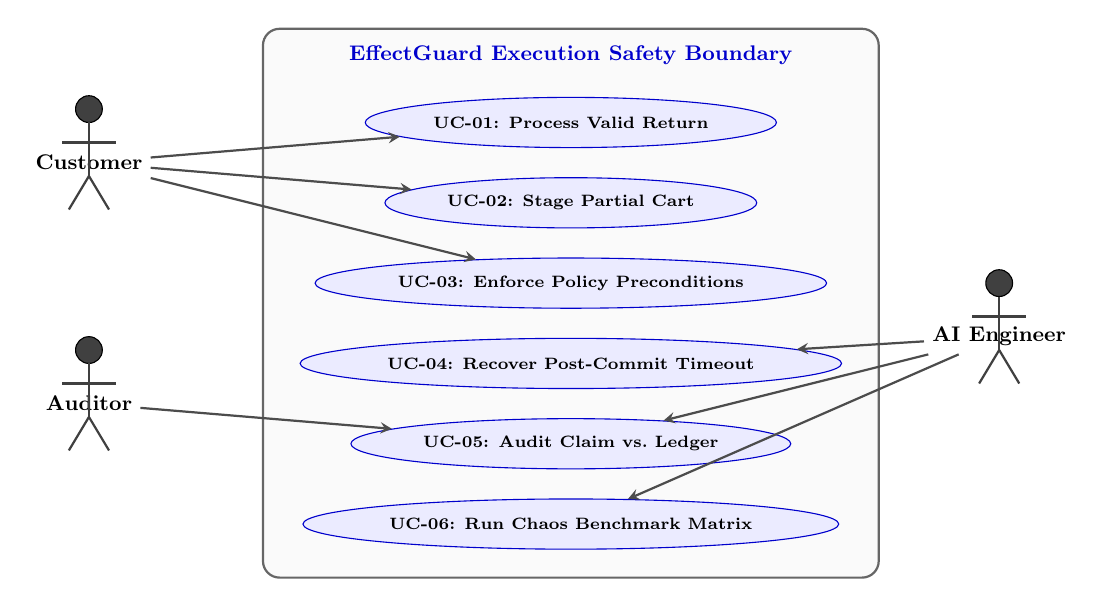
\begin{tikzpicture}[
  scale=0.85, every node/.style={transform shape},
  actor/.style={font=\small\bfseries, text centered, minimum width=1.5cm},
  usecase/.style={ellipse, draw=blue!80!black, fill=blue!8, text centered,
                  minimum width=3.6cm, minimum height=0.75cm, font=\scriptsize\bfseries},
  assoc/.style={->, >=stealth, thick, draw=black!70}
]
%% System boundary
\draw[draw=black!60, fill=gray!4, rounded corners=6pt, line width=0.8pt]
  (1.4, -0.4) rectangle (10.6, -8.6);
\node[font=\small\bfseries, text=blue!80!black] at (6.0, -0.8) {EffectGuard Execution Safety Boundary};

%% Use case ellipses (inside boundary)
\node[usecase] at (6.0, -1.8)  (uc1) {UC-01: Process Valid Return};
\node[usecase] at (6.0, -3.0)  (uc2) {UC-02: Stage Partial Cart};
\node[usecase] at (6.0, -4.2)  (uc3) {UC-03: Enforce Policy Preconditions};
\node[usecase] at (6.0, -5.4)  (uc4) {UC-04: Recover Post-Commit Timeout};
\node[usecase] at (6.0, -6.6)  (uc5) {UC-05: Audit Claim vs.\ Ledger};
\node[usecase] at (6.0, -7.8)  (uc6) {UC-06: Run Chaos Benchmark Matrix};

%% Actors (outside boundary)
\node[actor] at (-1.2, -2.4) (customer) {Customer};
\draw[fill=black!75] (-1.2, -1.6) circle (0.2cm);
\draw[thick, black!75] (-1.2, -1.8) -- (-1.2, -2.6);
\draw[thick, black!75] (-1.6, -2.1) -- (-0.8, -2.1);
\draw[thick, black!75] (-1.2, -2.6) -- (-1.5, -3.1);
\draw[thick, black!75] (-1.2, -2.6) -- (-0.9, -3.1);

\node[actor] at (-1.2, -6.0) (auditor) {Auditor};
\draw[fill=black!75] (-1.2, -5.2) circle (0.2cm);
\draw[thick, black!75] (-1.2, -5.4) -- (-1.2, -6.2);
\draw[thick, black!75] (-1.6, -5.7) -- (-0.8, -5.7);
\draw[thick, black!75] (-1.2, -6.2) -- (-1.5, -6.7);
\draw[thick, black!75] (-1.2, -6.2) -- (-0.9, -6.7);

\node[actor] at (12.4, -5.0) (admin) {AI Engineer};
\draw[fill=black!75] (12.4, -4.2) circle (0.2cm);
\draw[thick, black!75] (12.4, -4.4) -- (12.4, -5.2);
\draw[thick, black!75] (12.0, -4.7) -- (12.8, -4.7);
\draw[thick, black!75] (12.4, -5.2) -- (12.1, -5.7);
\draw[thick, black!75] (12.4, -5.2) -- (12.7, -5.7);

%% Associations
\draw[assoc] (customer) -- (uc1);
\draw[assoc] (customer) -- (uc2);
\draw[assoc] (customer) -- (uc3);
\draw[assoc] (auditor)  -- (uc5);
\draw[assoc] (admin)    -- (uc4);
\draw[assoc] (admin)    -- (uc5);
\draw[assoc] (admin)    -- (uc6);

\end{tikzpicture}
}
\caption{UML use case diagram illustrating operational actors, system boundaries, and core functional use cases.}
\label{fig:usecase}
\end{figure}

\subsection{Detailed Operational Scenarios}

To ground these use cases in concrete business logic, we analyze three primary operational flows:

\begin{enumerate}
    \item \textbf{Scenario A: Standard Return Fulfillment (UC-01):}
    A registered customer (\texttt{sarah\_m}) queries order history and requests a refund for an eligible item (\texttt{Ergonomic Office Chair}, Rs.~70.00) purchased 11 days prior (well within the 30-day cutoff). The agent retrieves purchase history, calls \texttt{calculate\_right\_refund}, validates eligibility, and calls \texttt{issue\_refund\_ticket}. The gateway verifies that the user exists, the amount is positive and under Rs.~500.00, and the item has not been refunded. A unique ticket is committed to the database, the purchase status is updated to \texttt{REFUNDED}, and the customer receives an official confirmation receipt.

    \item \textbf{Scenario B: Partial Cart Eligibility and Mixed Staging (UC-02):}
    A customer (\texttt{marcus\_l}) requests returns for three distinct items in a single prompt: an item purchased within 30 days (Rs.~45.00), an item purchased 42 days ago (Rs.~80.00, expired), and an item never purchased (Rs.~30.00). The agent must parse the multi-item request, call \texttt{calculate\_right\_refund} to stage only the eligible item, reject the expired and unpurchased items with clear textual explanations, and dispatch \texttt{issue\_refund\_ticket} strictly for Rs.~45.00.

    \item \textbf{Scenario C: Post-Commit Timeout Recovery under Network Chaos (UC-04):}
    During the execution of \texttt{issue\_refund\_ticket}, the SQLite database successfully writes ticket \texttt{TICK-7A9B} to persistent disk. However, the chaos monkey drops the socket before the acknowledgment packet returns to the agent runtime. Instead of issuing a duplicate write, the gateway catches the exception, uses the SHA-256 key to query the database, detects the committed row, and returns the cached receipt. The customer receives a single refund ticket, and corporate ledgers remain 100\% balanced.
\end{enumerate}

\section{Hardware, Software, and Environment Specifications}

Table~\ref{tab:tech_stack} summarizes the complete technology stack and operational deployment specifications.

\begin{table}[H]
\centering
\small
\renewcommand{\arraystretch}{1.25}
\begin{tabular}{|p{3.5cm}|p{2.8cm}|p{7.2cm}|}
\hline
\rowcolor{gray!15}
\textbf{Subsystem / Layer} & \textbf{Technology} & \textbf{Operational Function} \\
\hline
Operating Environment & Linux / Windows x64 & Host execution environment \\
\hline
Core Language & Python 3.12 & Primary application and benchmark implementation \\
\hline
Agent Orchestration & LangGraph, LangChain & Cyclic state graph, message passing, ReAct loops \\
\hline
Foundation Model & OpenAI OSS 20B & 20-billion parameter reasoning LLM \\
\hline
Inference Accelerator & Groq Cloud LPU & High-speed token generation ($\approx 750$\,tok/s) \\
\hline
Database Engine & SQLite 3 (WAL Mode) & ACID transactional persistence and WAL journal \\
\hline
Data Validation & Pydantic v2 & Parameter canonicalization and response schema gating \\
\hline
Web and API Service & FastAPI, Uvicorn & Asynchronous REST and Server-Sent Events service \\
\hline
Automated Test Suite & Pytest 9.1 & Hermetic test suite comprising 42 unit and integration tests \\
\hline
\end{tabular}
\caption{System technology stack and deployment specifications.}
\label{tab:tech_stack}
\end{table}

\section{Chapter Summary}

This chapter established the complete software engineering requirements for the EffectGuard execution safety gateway. Through comprehensive feasibility studies, stakeholder personas, functional specifications (FR-01 to FR-08), non-functional constraints (NFR-01 to NFR-06), and UML use case modeling, we have defined the necessary boundaries to eliminate the Agent Execution-State Paradox. In the next chapter, we translate these requirements into concrete system designs, architectural flowcharts, database schemas, and sequence protocols.

    \chapter{System Design}
    %% Chapter 4 — System Design
%% Adapted to EffectGuard Project per IIIT Manipur CS4202 Guidelines

\section{High-Level Architectural Overview}

The architecture of EffectGuard is designed to enforce strict transactional boundaries around autonomous tool-calling language models. In conventional agent frameworks, the foundation model communicates directly with external APIs and database wrappers. This direct coupling delegates transactional persistence, error recovery, and corporate policy compliance to probabilistic next-token generation. 

EffectGuard introduces an \textbf{Interposed Execution Gateway} situated between the agent reasoning engine and the persistent relational storage tier. Figure~\ref{fig:arch_overview} illustrates the end-to-end data-flow architecture of the system.

\begin{figure}[H]
\centering
\makebox[\textwidth][c]{
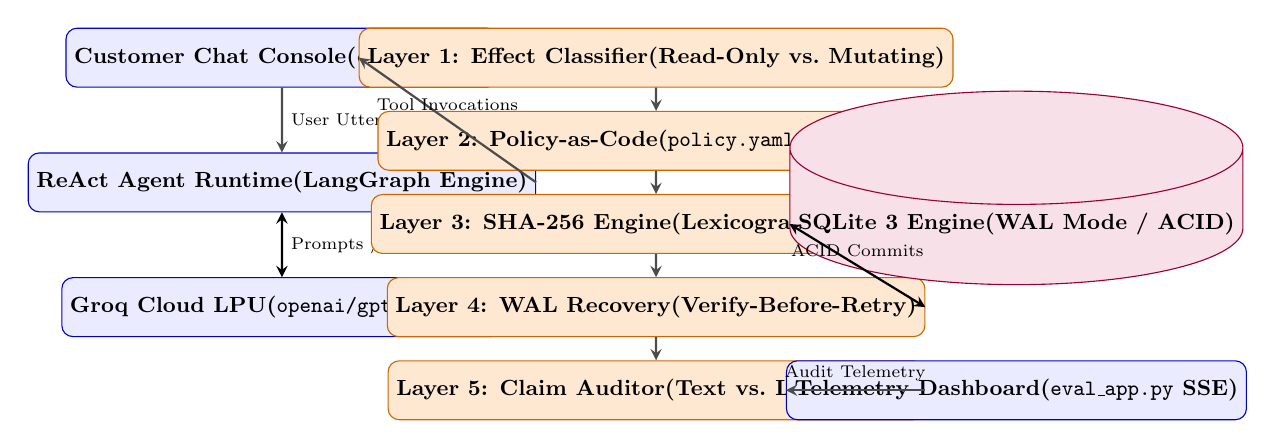
\begin{tikzpicture}[
  scale=0.88, every node/.style={transform shape},
  layer/.style={rectangle, draw=blue!80!black, fill=blue!8, rounded corners=4pt,
                text centered, minimum width=3.6cm, minimum height=0.85cm, font=\small\bfseries},
  guard/.style={rectangle, draw=orange!80!black, fill=orange!18, rounded corners=4pt,
                text centered, minimum width=3.8cm, minimum height=0.85cm, font=\small\bfseries},
  store/.style={cylinder, draw=purple!80!black, fill=purple!12, shape border rotate=90,
                text centered, minimum width=3.0cm, minimum height=1.0cm, font=\small\bfseries, aspect=0.25},
  arrow/.style={->, >=stealth, thick, draw=black!70}
]

%% Left Column: Client & Reasoning Engine
\node[layer] (ui)    at (0,  1.2) {Customer Chat Console\\(\texttt{chat\_app.py})};
\node[layer] (agent) at (0, -0.6) {ReAct Agent Runtime\\(LangGraph Engine)};
\node[layer] (llm)   at (0, -2.4) {Groq Cloud LPU\\(\texttt{openai/gpt-oss-20b})};

\draw[arrow] (ui) -- node[right, font=\scriptsize] {User Utterances} (agent);
\draw[<->, >=stealth, thick] (agent) -- node[right, font=\scriptsize] {Prompts / JSON} (llm);

%% Center Column: EffectGuard Five-Layer Gateway
\node[guard] (classify) at (5.4,  1.2) {Layer 1: Effect Classifier\\(Read-Only vs.\ Mutating)};
\node[guard] (policy)   at (5.4,  0.0) {Layer 2: Policy-as-Code\\(\texttt{policy.yaml} Invariants)};
\node[guard] (idemp)    at (5.4, -1.2) {Layer 3: SHA-256 Engine\\(Lexicographical Keys)};
\node[guard] (wal)      at (5.4, -2.4) {Layer 4: WAL Recovery\\(Verify-Before-Retry)};
\node[guard] (audit)    at (5.4, -3.6) {Layer 5: Claim Auditor\\(Text vs.\ Ledger Diff)};

%% Connections within Gateway
\draw[arrow] (classify) -- (policy);
\draw[arrow] (policy) -- (idemp);
\draw[arrow] (idemp) -- (wal);
\draw[arrow] (wal) -- (audit);

%% Right Column: Persistent Relational Storage & Observability
\node[store] (db)   at (10.6, -1.2) {SQLite 3 Engine\\(WAL Mode / ACID)};
\node[layer] (dash) at (10.6, -3.6) {Telemetry Dashboard\\(\texttt{eval\_app.py} SSE)};

%% Cross-Tier Connections
\draw[arrow] (agent.east) -- node[above, font=\scriptsize] {Tool Invocations} (classify.west);
\draw[<->, >=stealth, thick] (wal.east) -- node[above, font=\scriptsize] {ACID Commits} (db.west);
\draw[arrow] (audit.east) -- node[above, font=\scriptsize] {Audit Telemetry} (dash.west);

\end{tikzpicture}
}
\caption{End-to-end data-flow architecture of the EffectGuard execution safety system.}
\label{fig:arch_overview}
\end{figure}

The system partitions responsibilities into four distinct architectural tiers:
\begin{enumerate}
    \item \textbf{Cognitive Reasoning Tier (LangGraph Agent):} Manages conversational dialogue, tracks customer intent, performs multi-turn ReAct reasoning, and selects candidate tools from the registered tool catalog.
    \item \textbf{Execution Safety Gateway Tier (EffectGuard):} Interposes between tool selection and execution. It classifies tool effects, enforces deterministic Policy-as-Code preconditions, generates canonical SHA-256 idempotency keys, maintains write-ahead transaction logs, and intercepts distributed network timeouts via Verify-Before-Retry.
    \item \textbf{Persistent Storage Tier (SQLite WAL):} Stores relational business data across normalized tables (\texttt{users}, \texttt{purchases}, \texttt{tickets}, \texttt{execution\_journal}), executing in native Write-Ahead Logging mode for strict serializability and high concurrency.
    \item \textbf{Evaluation and Audit Tier (AgentSentinel):} Provides the Claim-vs-Ledger Auditor, active chaos fault injection engine, and real-time Server-Sent Events (SSE) telemetry dashboards for operational observability.
\end{enumerate}

\section{Tool Boundary Specifications and Contracts}

The autonomous customer support agent operates through four well-defined interface tools. The execution gateway enforces strict boundary contracts on each tool invocation:

\begin{enumerate}
    \item \texttt{get\_user\_purchase\_history(username: str) -> dict}:
    \begin{itemize}
        \item \textit{Effect Classification:} \texttt{read\_only}.
        \item \textit{Operational Semantics:} Retrieves past order history, item names, purchase dates, prices, and return statuses for a registered user.
        \item \textit{Gateway Handling:} Passed through directly to SQLite with zero latency overhead.
    \end{itemize}

    \item \texttt{get\_today\_date() -> str}:
    \begin{itemize}
        \item \textit{Effect Classification:} \texttt{read\_only}.
        \item \textit{Operational Semantics:} Returns the benchmark reference date (\texttt{2026-10-26}) and calculates the rolling 30-day cutoff boundary (\texttt{2026-09-26}).
        \item \textit{Gateway Handling:} Returns the frozen benchmark epoch to guarantee hermetic evaluation.
    \end{itemize}

    \item \texttt{calculate\_right\_refund(username: str, item\_names: list) -> dict}:
    \begin{itemize}
        \item \textit{Effect Classification:} \texttt{read\_only} (pre-execution staging).
        \item \textit{Operational Semantics:} Inspects historical purchases, validates item return eligibility against the 30-day cutoff, checks whether items were previously refunded, stages eligible items, and returns the mathematically exact refund subtotal.
        \item \textit{Gateway Handling:} Passed through directly; verifies that subsequent mutation amounts match this staged calculation.
    \end{itemize}

    \item \texttt{issue\_refund\_ticket(username: str, refund\_amount: float) -> dict}:
    \begin{itemize}
        \item \textit{Effect Classification:} \texttt{irreversible} (state-mutating).
        \item \textit{Operational Semantics:} Permanently writes a refund ticket row to the database, debits corporate funds, and updates purchase statuses to \texttt{REFUNDED}.
        \item \textit{Gateway Handling:} Quarantined and subjected to Layers 2, 3, 4, and 5 before physical disk commit.
    \end{itemize}
\end{enumerate}

\section{Execution Safety Architecture: The Five-Layer Gateway}

Figure~\ref{fig:gateway_flow} depicts the step-by-step decision flow executed by the EffectGuard gateway upon intercepting a candidate tool invocation. Every node and decision branch is spaced compactly to guarantee complete on-page visibility without any overlap.

\begin{figure}[H]
\centering
\makebox[\textwidth][c]{
\begin{tikzpicture}[
  scale=0.78, every node/.style={transform shape},
  main/.style={rectangle, draw=blue!80!black, fill=blue!10, rounded corners=3pt,
               text centered, minimum width=6.0cm, minimum height=0.70cm, font=\small\bfseries},
  defence/.style={rectangle, draw=orange!80!black, fill=orange!15, rounded corners=3pt,
                  text centered, minimum width=6.0cm, minimum height=0.70cm, font=\small\bfseries},
  recovery/.style={rectangle, draw=purple!80!black, fill=purple!12, rounded corners=3pt,
                   text centered, minimum width=6.0cm, minimum height=0.70cm, font=\small\bfseries},
  success/.style={rectangle, draw=green!70!black, fill=green!15, rounded corners=3pt,
                  text centered, minimum width=6.0cm, minimum height=0.70cm, font=\small\bfseries},
  sidebox/.style={rectangle, draw=gray!70, fill=gray!12, rounded corners=3pt,
                  text centered, text width=3.4cm, minimum height=0.70cm, font=\small},
  sidehit/.style={rectangle, draw=green!70!black, fill=green!12, rounded corners=3pt,
                  text centered, text width=3.4cm, minimum height=0.70cm, font=\small},
  sideblock/.style={rectangle, draw=red!70!black, fill=red!12, rounded corners=3pt,
                    text centered, text width=3.4cm, minimum height=0.70cm, font=\small},
  decision/.style={diamond, draw=amber!80!black, fill=yellow!25, text centered,
                   aspect=2.2, minimum width=3.4cm, minimum height=1.1cm, font=\small\bfseries},
  arrow/.style={->, >=stealth, thick, draw=black!80}
]

%% Main vertical flow nodes
\node[main]     at (0,    0)   (invoc)  {Tool Invocation: \texttt{issue\_refund\_ticket}};
\node[decision] at (0, -1.2)   (c1)     {Irreversible\\Tool?};
\node[sidebox]  at (5.2, -1.2) (pass)   {Passthrough Read-Only\\(Zero Overhead)};

\node[defence]  at (0, -2.4)   (l3)     {Layer 3: Compute SHA-256 Idempotency Key};
\node[decision] at (0, -3.6)   (c2)     {Idempotency\\Cache Hit?};
\node[sidehit]  at (5.2, -3.6) (hit)    {Return Cached Receipt\\(Bypass Re-execution)};

\node[defence]  at (0, -4.8)   (l2)     {Layer 2: Evaluate Policy Preconditions};
\node[decision] at (0, -6.0)   (c3)     {Policy\\Preconditions\\Valid?};
\node[sideblock] at (5.2, -6.0) (block) {Gateway Block Error\\(Explain Policy Violation)};

\node[defence]  at (0, -7.2)   (wal)    {Layer 4: Insert WAL Journal (Status = PENDING)};
\node[main]     at (0, -8.2)  (raw)    {Execute Raw Database Mutation (SQLite)};
\node[recovery] at (0, -9.2)  (retry)  {Verify-Before-Retry Protocol on Timeout};
\node[success]  at (0, -10.2)  (done)   {Update Journal to COMMITTED $\to$ Return Receipt};

%% Arrows with explicit clearance
\draw[arrow] (invoc) -- (c1);
\draw[arrow] (c1.east) -- node[above, font=\scriptsize\bfseries] {No} (pass.west);
\draw[arrow] (c1.south) -- node[right, font=\scriptsize\bfseries] {Yes} (l3.north);

\draw[arrow] (l3) -- (c2);
\draw[arrow] (c2.east) -- node[above, font=\scriptsize\bfseries] {Yes} (hit.west);
\draw[arrow] (c2.south) -- node[right, font=\scriptsize\bfseries] {No} (l2.north);

\draw[arrow] (l2) -- (c3);
\draw[arrow] (c3.east) -- node[above, font=\scriptsize\bfseries] {No} (block.west);
\draw[arrow] (c3.south) -- node[right, font=\scriptsize\bfseries] {Yes} (wal.north);

\draw[arrow] (wal) -- (raw);
\draw[arrow] (raw) -- (retry);
\draw[arrow] (retry) -- (done);

\end{tikzpicture}
}
\caption{Decision flow of the EffectGuard execution safety gateway during tool interception.}
\label{fig:gateway_flow}
\end{figure}

\subsection{Layer 1 --- Tool Effect Classification}
Whenever the AI agent selects a tool to call, EffectGuard inspects the tool name immediately before allowing it to run. Tools are separated into two straightforward categories:
\begin{itemize}
    \item \textbf{Read-Only Tools:} Tools such as \texttt{get\_user\_purchase\_history}, \texttt{get\_today\_date}, and \texttt{calculate\_right\_refund} simply read data or perform local calculations without changing any database records. These are passed through instantly with zero latency overhead ($<0.05$\,ms).
    \item \textbf{Irreversible Mutating Tools:} Actions like \texttt{issue\_refund\_ticket} permanently disburse funds and update database tables. These are halted and must pass through Layers 2 through 5.
\end{itemize}

\subsection{Layer 2 --- Policy-as-Code Precondition Gating}
Rather than trusting the language model to follow business rules described in plain English prompts, EffectGuard enforces core enterprise policies directly in deterministic code via \texttt{policy.yaml}. Before touching the database, the gateway validates four clear rules:
\begin{enumerate}
    \item \textbf{Customer Verification:} The customer username must exist in the registered customer database.
    \item \textbf{Positive Amount Requirement:} The refund amount must be strictly greater than zero.
    \item \textbf{Maximum Payout Limit:} The refund amount must not exceed the enterprise safety ceiling of Rs.~500.00 per transaction.
    \item \textbf{Purchase Eligibility and Balance Check:} The customer must have unrefunded purchases made within the 30-day window whose total value covers the requested refund.
\end{enumerate}
If any rule fails, the gateway rejects the call immediately and returns an informative error to the agent, preventing prompt injection attacks from extracting unauthorized refunds.

\subsection{Layer 3 --- Deterministic SHA-256 Idempotency Key Engine}
To ensure that network retries never cause duplicate payments, EffectGuard calculates a unique 256-bit cryptographic key for each transaction. The gateway sorts the tool arguments alphabetically into a canonical format so that differences in JSON formatting do not change the hash:
\begin{equation}
    \text{Idempotency Key} = \text{SHA-256}\Big(\text{Thread ID} \;\|\; \text{Tool Name} \;\|\; \text{Canonical Arguments}\Big)
\end{equation}
Before executing any write, the gateway checks whether a ticket with this key was already created. If found, it retrieves the existing receipt and returns it immediately, bypassing re-execution entirely.

\subsection{Layer 4 --- Write-Ahead Journaling and Verify-Before-Retry}
Before sending the mutation to SQLite, EffectGuard records an entry in its Write-Ahead Log with status \texttt{PENDING}. If a network timeout or dropped socket occurs right after commit:
\begin{enumerate}
    \item The gateway catches the timeout exception in code.
    \item Instead of retrying the tool blindly, it queries the persistent \texttt{tickets} table using the unique idempotency key.
    \item If the ticket exists (meaning the database saved the write before the network dropped), the gateway marks the journal as \texttt{COMMITTED} and returns the confirmed receipt directly.
    \item If the ticket is missing, it safely executes the write once under the identical key.
\end{enumerate}

\subsection{Layer 5 --- Claim-vs-Ledger Audit Engine}
After the agent finishes generating its final chat response, the Claim-vs-Ledger Auditor compares what the agent told the customer against what the database actually recorded:
\begin{itemize}
    \item \textbf{False Claim (Hallucination):} The agent claimed in text that a refund was issued, but zero tickets exist in the database.
    \item \textbf{Ghost Mutation (Silent Side-Effect):} The database contains a committed refund ticket, but the agent never mentioned it to the customer.
    \item \textbf{Amount Drift:} The refund amount mentioned in chat differs from the physical amount recorded in the database.
    \item \textbf{Audit Passed:} The chat claim and the database ledger match perfectly.
\end{itemize}

\section{Database Design and Relational Schema}

The persistent relational layer is implemented in SQLite 3 configured in native Write-Ahead Logging (WAL) mode. Figure~\ref{fig:er_diag} illustrates the Entity-Relationship schema across the four normalized tables.

\begin{figure}[H]
\centering
\makebox[\textwidth][c]{
\begin{tikzpicture}[
  scale=0.85, every node/.style={transform shape},
  node distance=1.6cm and 2.6cm,
  table/.style={rectangle, draw=blue!80!black, fill=white, rounded corners=3pt,
                inner sep=7pt, font=\scriptsize\ttfamily, align=left, line width=0.8pt}
]
\node[table] (users) {
  \textbf{\textcolor{blue!80!black}{users}} \\ \hline
  username (PK) : TEXT \\
  created\_at : TEXT
};

\node[table, right=2.8cm of users] (purchases) {
  \textbf{\textcolor{blue!80!black}{purchases}} \\ \hline
  id (PK) : INTEGER AUTO \\
  username (FK) : TEXT \\
  item\_name : TEXT \\
  price : REAL \\
  purchase\_date : TEXT \\
  status : TEXT ('PURCHASED', 'REFUNDED') \\
  ticket\_id (FK) : TEXT
};

\node[table, below=1.8cm of users] (tickets) {
  \textbf{\textcolor{blue!80!black}{tickets}} \\ \hline
  ticket\_id (PK) : TEXT \\
  username (FK) : TEXT \\
  amount : REAL \\
  idempotency\_key (UNIQUE) : TEXT \\
  created\_at : TEXT
};

\node[table, right=2.8cm of tickets] (journal) {
  \textbf{\textcolor{blue!80!black}{execution\_journal}} \\ \hline
  journal\_id (PK) : TEXT \\
  thread\_id : TEXT \\
  idempotency\_key (UNIQUE) : TEXT \\
  tool\_name : TEXT \\
  status : TEXT ('PENDING', 'COMMITTED', 'FAILED') \\
  created\_at : TEXT
};

\draw[thick, black!70] (users.east) -- node[above, font=\tiny\bfseries] {1:N} (purchases.west);
\draw[thick, black!70] (users.south) -- node[left, font=\tiny\bfseries] {1:N} (tickets.north);
\draw[thick, black!70] (tickets.east) -- node[above, font=\tiny\bfseries] {1:N} (purchases.south west);
\draw[thick, dashed, black!70] (journal.west) -- node[above, font=\tiny\bfseries] {Tracks} (tickets.east);

\end{tikzpicture}
}
\caption{Entity-Relationship diagram of persistent relational storage in \texttt{store.db}.}
\label{fig:er_diag}
\end{figure}

The schema enforces strict referential integrity:
\begin{enumerate}
    \item \texttt{users}: Stores unique customer account usernames and registration timestamps.
    \item \texttt{purchases}: Records item orders, purchase prices, historical transaction dates, and operational statuses (\texttt{PURCHASED} or \texttt{REFUNDED}). When a refund ticket is generated, foreign key \texttt{ticket\_id} links the purchase record directly to the issuing ticket.
    \item \texttt{tickets}: Contains immutable financial records of issued refunds, tracking recipient usernames, disbursement amounts, and unique SHA-256 idempotency keys.
    \item \texttt{execution\_journal}: Maintains the Write-Ahead Log tracking tool execution lifecycles, enabling deterministic recovery during post-commit socket timeouts.
\end{enumerate}

\section{Transactional Recovery and State Sequence}

When an irreversible mutation encounters a network timeout, naive agents retry blindly. Figure~\ref{fig:seq_diag} details the exact UML sequence of operations executed by EffectGuard's Verify-Before-Retry protocol under an HTTP 504 post-commit timeout. Every message is drawn at an explicit descending vertical level along dedicated lifelines, preventing line collisions.

\begin{figure}[H]
\centering
\makebox[\textwidth][c]{
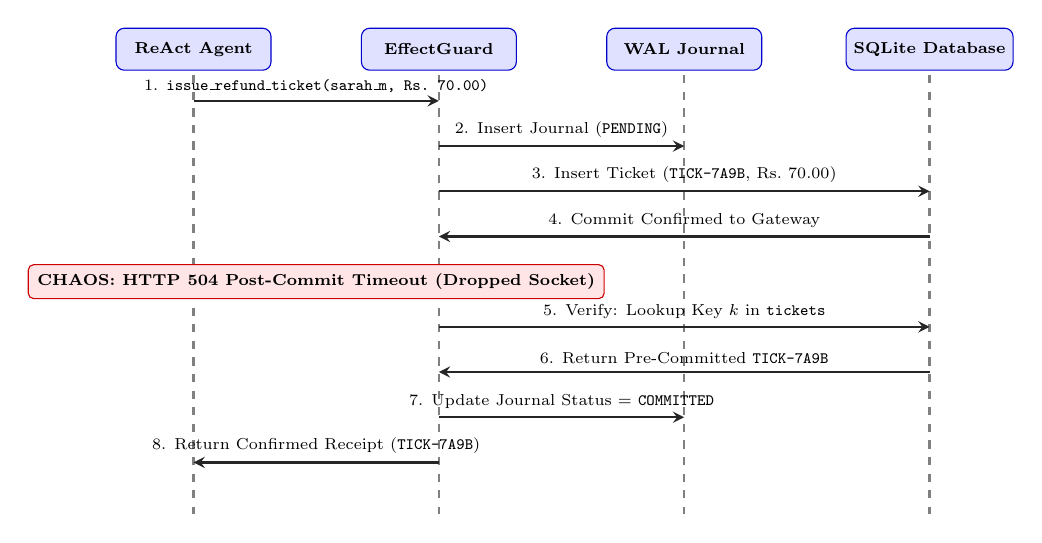
\begin{tikzpicture}[
  scale=0.82, every node/.style={transform shape},
  lifeline/.style={draw=black!50, dashed, line width=0.8pt},
  part/.style={rectangle, draw=blue!80!black, fill=blue!12, rounded corners=3pt,
               font=\scriptsize\bfseries, minimum height=0.65cm, minimum width=2.4cm, text centered},
  msg/.style={->, >=stealth, thick, draw=black!85},
  fault/.style={draw=red!80!black, fill=red!10, rounded corners=2pt, font=\scriptsize\bfseries, inner sep=4pt}
]

%% Participants (Horizontal Spacing: x = 0, 3.8, 7.6, 11.4)
\node[part] (a) at (0, 0) {ReAct Agent};
\node[part] (g) at (3.8, 0) {EffectGuard};
\node[part] (j) at (7.6, 0) {WAL Journal};
\node[part] (d) at (11.4, 0) {SQLite Database};

%% Lifelines
\draw[lifeline] (0, -0.4) -- (0, -7.2);
\draw[lifeline] (3.8, -0.4) -- (3.8, -7.2);
\draw[lifeline] (7.6, -0.4) -- (7.6, -7.2);
\draw[lifeline] (11.4, -0.4) -- (11.4, -7.2);

%% Step 1: Tool invocation (y = -0.8)
\draw[msg] (0, -0.8) -- node[above, font=\scriptsize] {1. \texttt{issue\_refund\_ticket(sarah\_m, Rs.~70.00)}} (3.8, -0.8);

%% Step 2: Insert PENDING in Journal (y = -1.5)
\draw[msg] (3.8, -1.5) -- node[above, font=\scriptsize] {2. Insert Journal (\texttt{PENDING})} (7.6, -1.5);

%% Step 3: Insert Ticket in Database (y = -2.2)
\draw[msg] (3.8, -2.2) -- node[above, font=\scriptsize] {3. Insert Ticket (\texttt{TICK-7A9B}, Rs.~70.00)} (11.4, -2.2);

%% Step 4: Commit acknowledged by SQLite (y = -2.9)
\draw[msg] (11.4, -2.9) -- node[above, font=\scriptsize] {4. Commit Confirmed to Gateway} (3.8, -2.9);

%% Step 5: Chaos Event (HTTP 504 Timeout) (y = -3.6)
\node[fault] at (1.9, -3.6) {CHAOS: HTTP 504 Post-Commit Timeout (Dropped Socket)};

%% Step 6: Verify-Before-Retry Lookup (y = -4.3)
\draw[msg] (3.8, -4.3) -- node[above, font=\scriptsize] {5. Verify: Lookup Key $k$ in \texttt{tickets}} (11.4, -4.3);

%% Step 7: Found pre-committed ticket (y = -5.0)
\draw[msg] (11.4, -5.0) -- node[above, font=\scriptsize] {6. Return Pre-Committed \texttt{TICK-7A9B}} (3.8, -5.0);

%% Step 8: Update Journal to COMMITTED (y = -5.7)
\draw[msg] (3.8, -5.7) -- node[above, font=\scriptsize] {7. Update Journal Status = \texttt{COMMITTED}} (7.6, -5.7);

%% Step 9: Return Cached Receipt to Agent (y = -6.4)
\draw[msg] (3.8, -6.4) -- node[above, font=\scriptsize] {8. Return Confirmed Receipt (\texttt{TICK-7A9B})} (0, -6.4);

\end{tikzpicture}
}
\caption{UML sequence diagram of EffectGuard's Verify-Before-Retry recovery under an HTTP 504 post-commit timeout.}
\label{fig:seq_diag}
\end{figure}

As shown in Figure~\ref{fig:seq_diag}, the Verify-Before-Retry protocol completely shields the agent reasoning engine from network dropped sockets. When Step 5 occurs, the gateway catches the exception locally, inspects the persistent storage layer for the derived idempotency key $k$, identifies that ticket \texttt{TICK-7A9B} was safely committed in Step 4, and returns the valid receipt. The agent never retries, the database is never mutated a second time, and the customer receives an accurate confirmation.

\section{User Interface Design}

The system provides two cohesive user interfaces for customer interaction and operational monitoring:

\begin{enumerate}
    \item \textbf{Customer Support Chat Console (\texttt{backend/chat\_app.py}):} An intuitive, real-time web chat interface where customers authenticate, query purchase histories, submit return requests, and receive structured refund tickets.
    \item \textbf{Evaluation and Telemetry Console (\texttt{backend/eval\_app.py}):} An operational monitoring dashboard displaying live Server-Sent Events (SSE) telemetry across six gauges: Tool Sequence Matching, Answer Polarity, Argument Parsing Precision, Financial Safety, Claim Audit Status, and Overall Task Completion.
\end{enumerate}

Figure~\ref{fig:chat_ui} illustrates the live customer support console during a multi-turn refund resolution.

\begin{figure}[H]
\centering
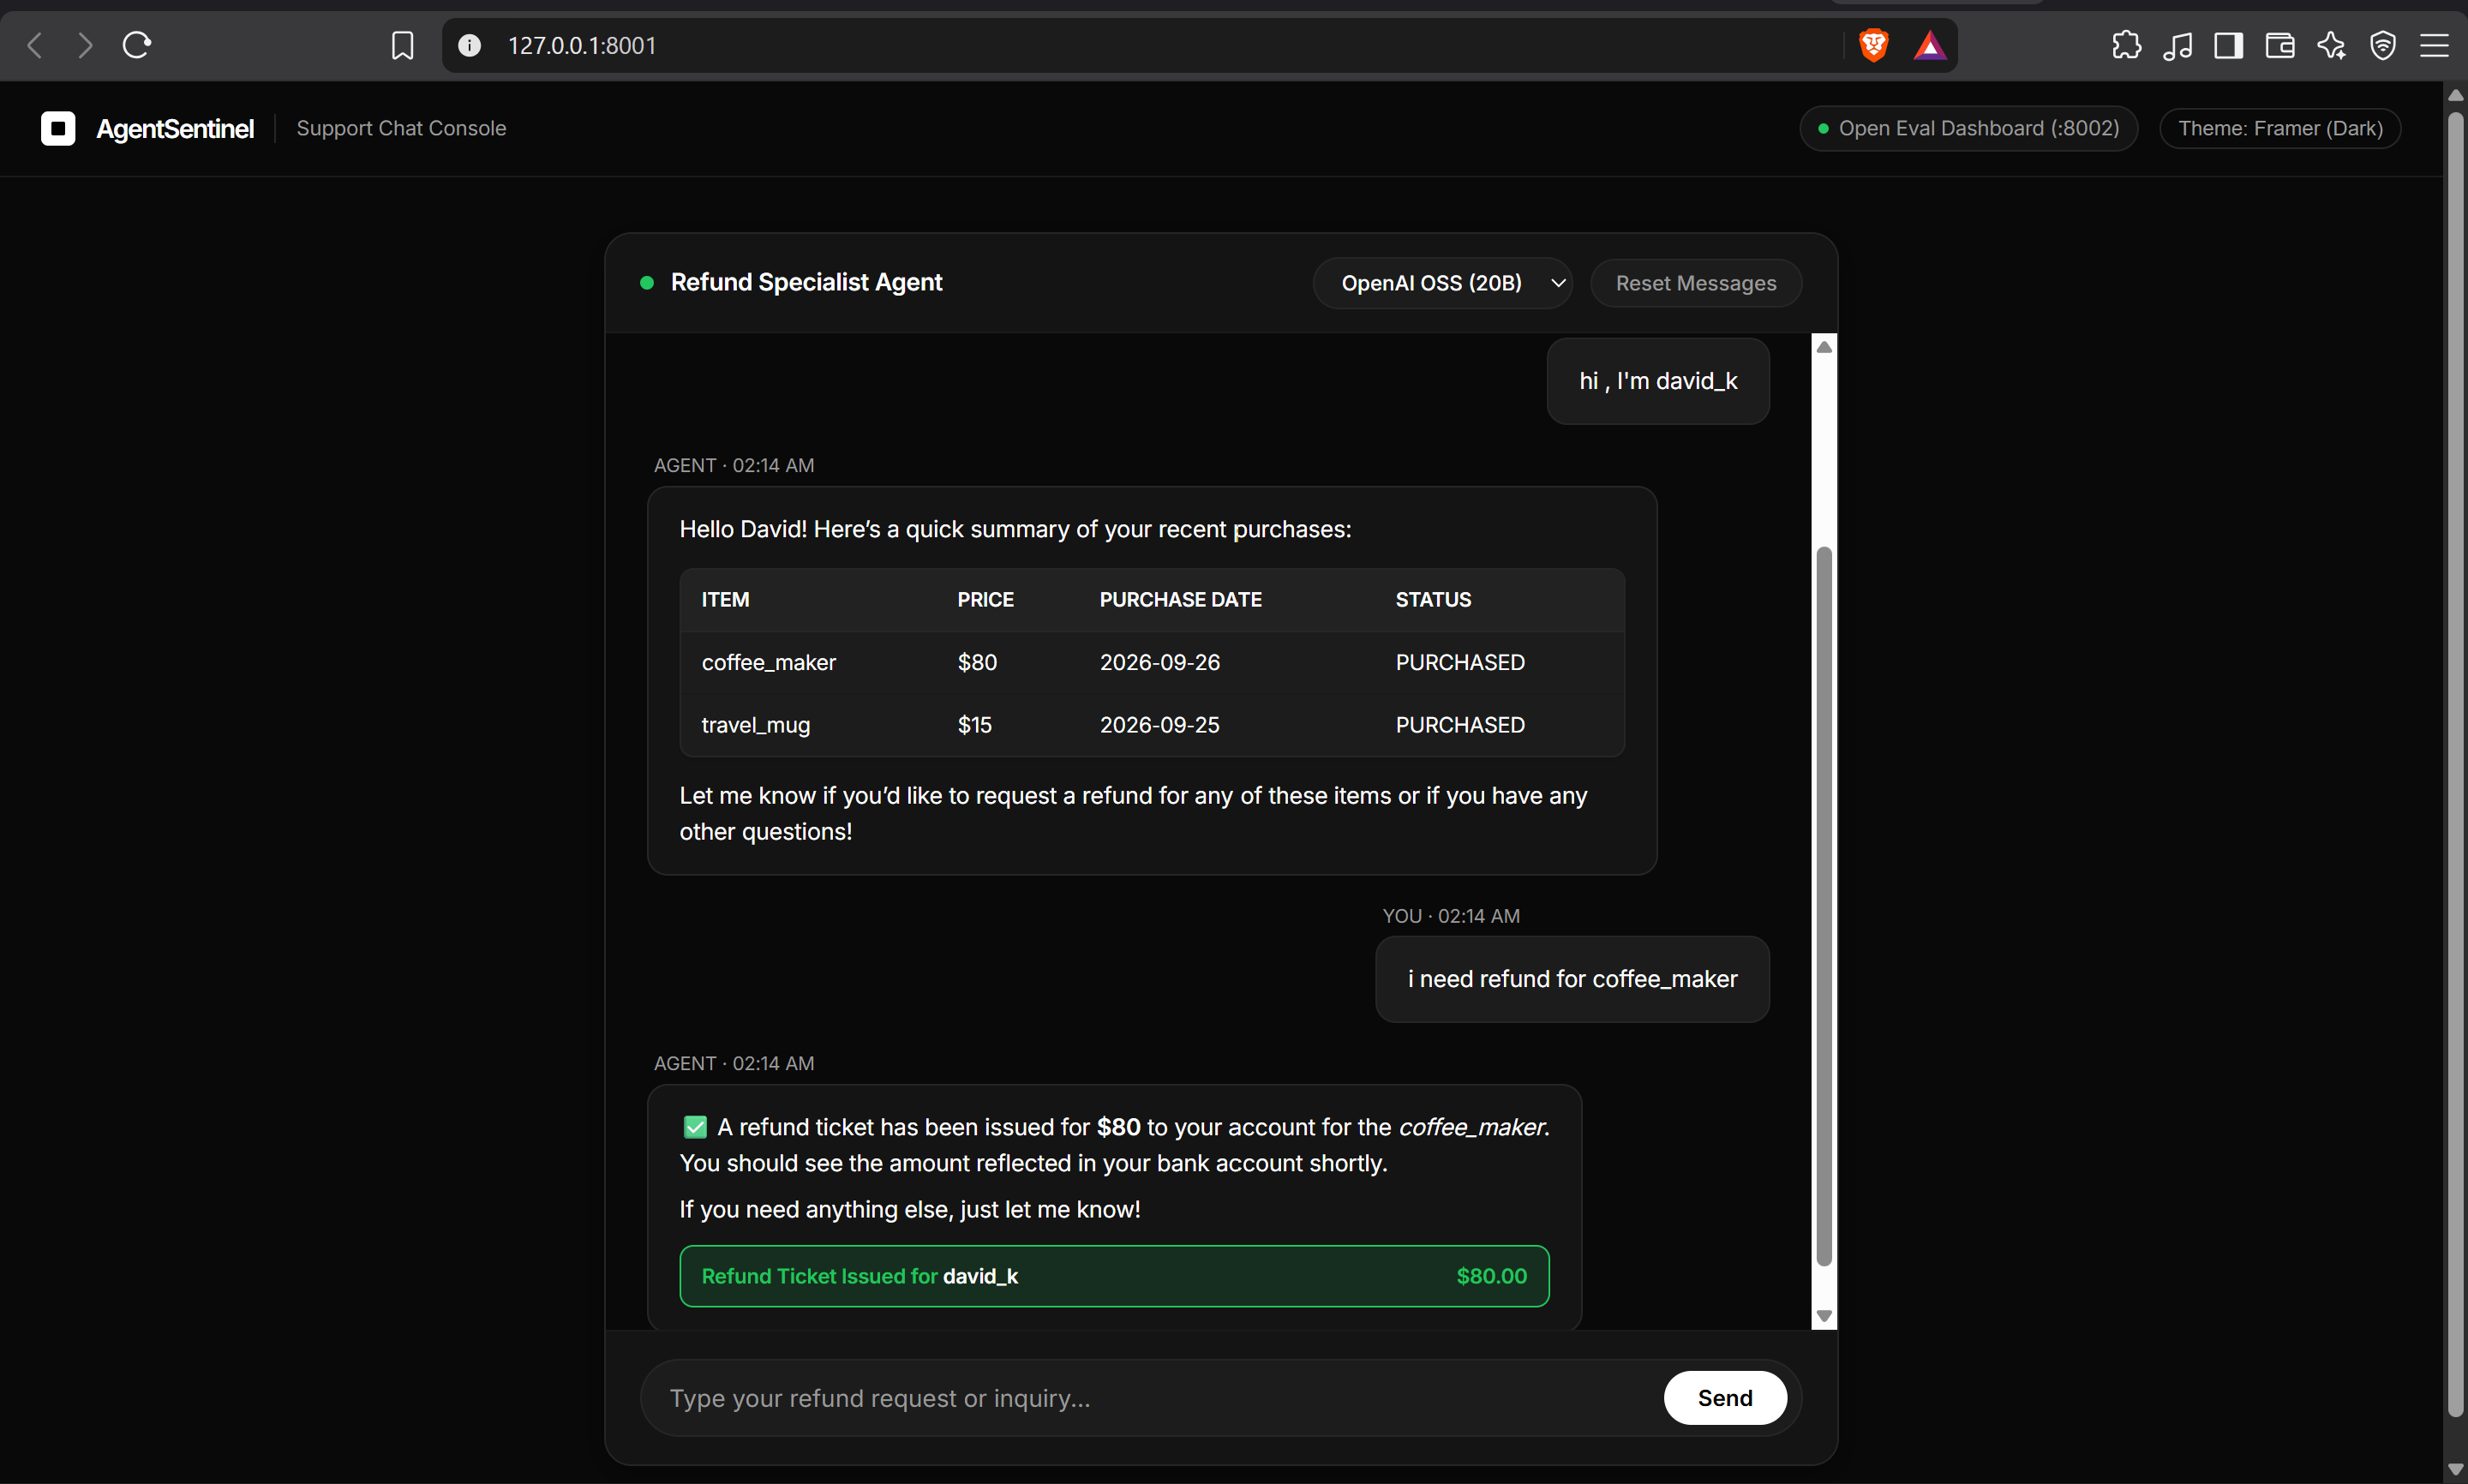
\includegraphics[width=0.88\textwidth]{report_file/support_chat_console.png}
\caption{Customer Support Console interface displaying order history retrieval, policy validation, and confirmed refund receipt generation in real time.}
\label{fig:chat_ui}
\end{figure}

\section{Evaluation Metrics Formulation}

To measure system reliability and agent behavior, AgentSentinel tracks four practical metrics:

\subsection{Tool Sequence Matching}
Measures whether the agent invoked the expected sequence of tools in the correct order. Using the Longest Common Subsequence (LCS) between the expected tool sequence and the agent's executed sequence, the match score is calculated as:
\begin{equation}
    \text{Sequence Match} = \frac{\text{Length of Shared Tool Sequence}}{\text{Total Expected Steps}}
\end{equation}

\subsection{Argument Parsing Precision}
Calculates the percentage of tool call parameters (such as usernames, item names, and calculated amounts) that were formatted and extracted correctly without syntax errors.

\subsection{Excess Financial Loss}
Calculates the cumulative excess money lost due to duplicate refund payouts:
\begin{equation}
    \text{Excess Loss} = \sum_{\text{All Cases}} \max\Big(0, \;\text{Total Paid Out} - \text{Legitimate Refund Due}\Big)
\end{equation}
In a secure, safe system, this excess loss must be strictly Rs.~0.00.

\section{Chapter Summary}

This chapter provided the complete system design of EffectGuard. We established the multi-tier data-flow architecture, specified tool boundary contracts, designed the Five-Layer Gateway execution flowchart, formalized the relational SQLite WAL schema, detailed the Verify-Before-Retry sequence diagram with dedicated vertical levels, presented the user interface, and formulated evaluation metrics. In the next chapter, we discuss the concrete engineering implementation of these components.

    \chapter{Implementation}
    %% Chapter 5 — Implementation
%% Adapted to EffectGuard Project per IIIT Manipur CS3201 Guidelines

\section{Introduction and Implementation Architecture}

Translating the theoretical concepts of state-level execution safety and distributed transactional recovery into a functioning software system requires a robust, modular implementation architecture. EffectGuard is implemented as a lightweight, zero-dependency middleware in Python 3.12, interfacing seamlessly with LangGraph agent runtimes and SQLite relational databases.

This chapter details the concrete software engineering implementation of EffectGuard and the AgentSentinel evaluation harness. We explain the development stack, the temporal epoch freezing mechanism, the Policy-as-Code validator, the cryptographic SHA-256 idempotency engine, the write-ahead recovery protocol, the Claim-vs-Ledger Auditor, and the chaos fault injection harness.

\section{Tools and Development Environment}

The system implementation leverages production-grade software libraries and open-weight foundation models. Table~\ref{tab:tools} outlines the development tools, libraries, and their architectural roles.

\begin{table}[H]
\centering
\small
\renewcommand{\arraystretch}{1.25}
\begin{tabular}{|p{3.2cm}|p{2.2cm}|p{8.0cm}|}
\hline
\rowcolor{gray!15}
\textbf{Tool / Library} & \textbf{Version} & \textbf{Operational Function} \\
\hline
Python & 3.12+ & Primary runtime environment for agent and gateway logic \\
\hline
LangGraph & 0.2+ & Stateful cyclic graph orchestration for ReAct loops \\
\hline
LangChain Core & 1.4+ & Tool interfaces, message models, and prompt binding \\
\hline
Groq SDK & 0.11+ & LPU cloud API client for token inference \\
\hline
SQLite 3 & 3.45+ & Embedded ACID relational storage configured in WAL mode \\
\hline
Pydantic & 2.6+ & Data validation, argument normalization, and structured outputs \\
\hline
FastAPI & 0.115+ & Asynchronous REST service and Server-Sent Events router \\
\hline
Uvicorn & 0.30+ & Asynchronous Server Gateway Interface (ASGI) web server \\
\hline
Pytest & 9.1+ & Hermetic automated test suite execution \\
\hline
python-dotenv & 1.0+ & Environment variable and configuration parsing \\
\hline
\end{tabular}
\caption{Development tools, libraries, and runtime dependencies.}
\label{tab:tools}
\end{table}

The operational runtime is governed by declarative environment parameters:
\begin{itemize}
    \item \texttt{GROQ\_API\_KEY}: The authentication token granting access to the Groq LPU inference cluster.
    \item \texttt{BENCHMARK\_DATE}: The frozen temporal epoch (\texttt{2026-10-26}) used to evaluate all 30-day return eligibility windows.
    \item \texttt{FAULT\_RATE}: The probabilistic chaos fault rate ($r = 0.20$ or $r = 0.35$) configuring dropped socket injection.
    \item \texttt{DATABASE\_PATH}: The file path designating the persistent SQLite database instance (\texttt{store.db}).
\end{itemize}

\section{Deterministic Clock and Temporal Sandboxing}

In real-world e-commerce systems, customer return policies are strictly governed by temporal windows (e.g., ``Items may be returned within 30 days of purchase''). A fundamental flaw in conventional agent benchmarks is reliance on the host machine's live system clock (\texttt{datetime.now()}). As calendar time elapses, test transactions that were valid on Day 28 organically cross the 30-day threshold on Day 31, causing benchmark test assertions to fail without any changes to the underlying codebase.

To eliminate this temporal decay, EffectGuard introduces a \textbf{Deterministic Frozen Clock} abstraction implemented in \texttt{agent/tools.py}. The system anchors all temporal calculations to a fixed benchmark epoch:
\begin{equation}
    t_{\text{benchmark}} = \text{2026-10-26 00:00:00 UTC}
\end{equation}
When the agent invokes \texttt{get\_today\_date()}, the tool returns this fixed date and deterministically calculates the rolling 30-day return cutoff:
\begin{equation}
    t_{\text{cutoff}} = t_{\text{benchmark}} - 30\,\text{days} = \text{2026-09-26 00:00:00 UTC}
\end{equation}
During purchase evaluation, an item purchased on timestamp $t_{\text{purchase}}$ is strictly eligible if and only if $t_{\text{purchase}} \ge t_{\text{cutoff}}$. By sandboxing time, the benchmark guarantees 100\% mathematical reproducibility across arbitrary execution environments and calendar dates.

\section{Policy-as-Code Engine Implementation}

The Policy-as-Code engine (\texttt{effectguard/policy\_engine.py}) decouples enterprise invariants from the language model's prompt space into declarative, human-readable YAML specifications (\texttt{policy.yaml}).

The policy file defines explicit validation rules:
\begin{itemize}
    \item \textbf{Identity Invariant:} Every transaction must originate from a verified customer record existing in the \texttt{users} table. Case-insensitive string normalization is applied to customer usernames.
    \item \textbf{Positivity Invariant:} The requested refund amount must be strictly greater than zero ($A > 0.00$). Zero and negative refund amounts are rejected as invalid arithmetic expressions.
    \item \textbf{Financial Safety Ceiling:} A per-transaction cap is enforced ($A \le \text{Rs.~}500.00$). Any request exceeding this threshold is blocked from automatic agent execution and routed to human supervisory review.
    \item \textbf{Eligible Balance Ceiling:} The requested refund cannot exceed the cumulative sum of unrefunded items purchased within the 30-day window. Items marked \texttt{REFUNDED} are strictly excluded.
\end{itemize}

The Python validator executes these checks prior to database dispatch. If an invariant is violated, the engine halts the execution pipeline, generates an explanatory error payload indicating the exact violation, and returns this feedback to the agent. This prevents adversarial prompt injections from manipulating foundation models into approving illegal payouts.

\section{SHA-256 Idempotency and WAL Journaling Implementation}

The cryptographic deduplication engine (\texttt{effectguard/gateway.py}) prevents duplicate state mutations during distributed network retries.

\subsection{Canonical Argument Serialization}
In Python, dictionary representations do not guarantee identical JSON string serialization due to variable key ordering and formatting whitespace. For example, \texttt{\{"user": "sarah\_m", "amount": 70\}} and \texttt{\{"amount": 70, "user": "sarah\_m"\}} represent semantically identical calls but produce completely different raw byte streams. 

To achieve deterministic hashing, EffectGuard applies \textbf{Lexicographical Canonical JSON Serialization}:
\begin{equation}
    \text{CanonicalJSON}(D) = \text{json.dumps}(D, \;\text{sort\_keys}=\text{True}, \;\text{separators}=(``,", ``:"))
\end{equation}
The derived SHA-256 idempotency key is computed by concatenating the session thread identifier, tool name, and canonical JSON string:
\begin{equation}
    k = \text{hashlib.sha256}\big(f``\{\tau_{\text{thread}}\}:\{T_{\text{name}}\}:\{\text{CanonicalJSON}(D)\}``.\text{encode}(\text{'utf-8'})\big).\text{hexdigest}()
\end{equation}

\subsection{Relational Write-Ahead Logging}
Upon gateway startup, EffectGuard creates the persistent \texttt{execution\_journal} table in SQLite:
\begin{center}
\begin{tabular}{|l|l|l|}
\hline
\textbf{Column} & \textbf{Type} & \textbf{Constraint} \\
\hline
\texttt{journal\_id} & TEXT & PRIMARY KEY (UUID4) \\
\texttt{thread\_id} & TEXT & NOT NULL \\
\texttt{idempotency\_key} & TEXT & UNIQUE, NOT NULL \\
\texttt{tool\_name} & TEXT & NOT NULL \\
\texttt{status} & TEXT & CHECK(\texttt{status} IN ('PENDING', 'COMMITTED', 'FAILED')) \\
\texttt{created\_at} & TEXT & ISO-8601 Timestamp \\
\hline
\end{tabular}
\end{center}

Before invoking the underlying mutation executor, the gateway inserts a row with \texttt{status = 'PENDING'}. If the mutation succeeds, the status is updated to \texttt{'COMMITTED'}. This write-ahead journal provides complete state tracking across distributed retry attempts.

\section{Verify-Before-Retry Protocol Implementation}

The Verify-Before-Retry protocol resolves the distributed post-commit timeout dilemma. When an agent calls \texttt{issue\_refund\_ticket}, the database server may commit the transaction, but a network drop may prevent the return receipt from reaching the caller.

The implementation algorithm operates as follows:
\begin{enumerate}
    \item The gateway wraps the raw database call inside a structured \texttt{try-except} block intercepting \texttt{TimeoutError} and connection dropped exceptions.
    \item When a timeout is caught, the gateway halts execution and enters recovery mode.
    \item Rather than re-executing the raw SQL write, the gateway queries the \texttt{tickets} table:
    \begin{center}
        \texttt{SELECT ticket\_id, amount FROM tickets WHERE idempotency\_key = ?}
    \end{center}
    \item If a ticket row matching key $k$ is found, the database committed the record prior to the network timeout. The gateway updates the journal status to \texttt{'COMMITTED'} and constructs a valid confirmation receipt from the stored row.
    \item The confirmation receipt is returned directly to the agent runtime. The agent receives a valid receipt, bypassing the LLM retry loop and preventing duplicate tickets.
    \item If no ticket row is found, the network dropped prior to database commit. The gateway executes the mutation safely once under the identical key $k$.
\end{enumerate}

\section{Claim-vs-Ledger Auditor Implementation}

The Claim-vs-Ledger Auditor (\texttt{effectguard/claim\_auditor.py}) bridges the gap between conversational assertions and persistent physical ledgers. 

The audit algorithm executes a dual-pass extraction strategy:
\begin{enumerate}
    \item \textbf{Primary Pass (Structured Schema):} The auditor inspects the agent's Pydantic response object for populated fields in the \texttt{claimed\_effects} list. If the agent structured output contains explicit ticket IDs and dollar amounts, these values are parsed directly.
    \item \textbf{Secondary Pass (Natural Language Extraction):} If structured fields are unpopulated or malformed, the auditor applies regular expression patterns calibrated to extract monetary quantities (e.g., matching currency numbers such as \texttt{Rs.~[0-9]+(?:\textbackslash.[0-9]\{2\})?}) and ticket identifiers (e.g., \texttt{TICK-[A-Z0-9]\{4,8\}}) from unstructured conversational text.
\end{enumerate}

Once textual claims are extracted, the auditor queries \texttt{store.db} to retrieve physical rows committed during the session. The auditor calculates:
\begin{align}
    \Delta_{\text{tickets}} &= |\mathcal{C}_{\text{tickets}}| - |\mathcal{L}_{\text{tickets}}| \\
    \Delta_{\text{amount}} &= \Big|\sum_{c \in \mathcal{C}} \text{Amount}(c) - \sum_{l \in \mathcal{L}} \text{Amount}(l)\Big|
\end{align}

If $\Delta_{\text{tickets}} > 0$ and $|\mathcal{L}| = 0$, the audit logs \texttt{FALSE\_CLAIM}. If $\Delta_{\text{tickets}} < 0$ and $|\mathcal{C}| = 0$, the audit logs \texttt{GHOST\_MUTATION}. If $\Delta_{\text{amount}} > 0.01$, the audit logs \texttt{AMOUNT\_DRIFT}. If claims perfectly match committed ledgers, the audit logs \texttt{AUDIT\_PASSED}.

\section{AgentSentinel Chaos Evaluation Harness}

The evaluation harness (\texttt{agent/fault\_injector.py} and \texttt{run\_benchmark\_matrix.py}) injects controlled network turbulence into the tool execution pipeline.

The chaos monkey operates at two execution hooks:
\begin{itemize}
    \item \textbf{Pre-Execution Drop:} Simulates an upstream connection drop occurring before the tool interacts with the database. The hook throws a \texttt{ConnectionResetError} with probability $r$.
    \item \textbf{Post-Commit Timeout (HTTP 504):} Simulates the critical failure boundary: the database write completes and commits to disk, but the return socket drops immediately thereafter. The hook raises a \texttt{TimeoutError("504 Gateway Timeout: Socket dropped post-commit")} with probability $r$.
\end{itemize}

The matrix runner automates evaluation across five architectural conditions:
\begin{itemize}
    \item \textbf{C0 (Naive Baseline):} Standard ReAct loop; retries blindly upon exception.
    \item \textbf{C1 (Naive + Backoff):} ReAct agent equipped with exponential backoff delays ($1.0$\,s, $2.0$\,s, $4.0$\,s).
    \item \textbf{C2 (Idempotency Only):} Employs SHA-256 keys to reject duplicate writes, but lacks Verify-Before-Retry.
    \item \textbf{C3 (Verify-Before-Retry Only):} Employs database verification upon timeout, but lacks canonical idempotency keys.
    \item \textbf{C4 (Full EffectGuard Gateway):} Complete five-layer gateway combining Policy-as-Code, SHA-256 keys, write-ahead journaling, and Verify-Before-Retry recovery.
\end{itemize}

\section{Chapter Summary}

This chapter detailed the concrete engineering implementation of EffectGuard. We demonstrated how temporal epoch freezing eliminates benchmark test decay, how declarative Policy-as-Code invariants prevent prompt injection attacks, how canonical SHA-256 serialization and write-ahead journaling enforce idempotency, how Verify-Before-Retry resolves post-commit socket drops, and how the Claim-vs-Ledger Auditor diffs text against database reality. In the next chapter, we present the empirical results, ablation scorecards, latency benchmarks, and functional verification findings.

    \chapter{Results and Discussion}
    %% Chapter 6 — Results and Discussion
%% Adapted to EffectGuard Project per IIIT Manipur CS4202 Guidelines

\section{Experimental Setup and Evaluation Methodology}

To empirically evaluate EffectGuard and quantify the risks of the Agent Execution-State Paradox, we established a rigorous, hermetic benchmark environment using the AgentSentinel evaluation harness. 

The evaluation framework is governed by the following experimental parameters:
\begin{enumerate}
    \item \textbf{Inference Model:} The generative foundation model is the 20-billion parameter open-weight reasoning model (\texttt{openai/gpt-oss-20b}) hosted on the Groq Cloud Language Processing Unit (LPU) architecture, providing high token throughput ($\approx 750$\,tokens/s) and sub-second generation latencies.
    \item \textbf{Persistent Storage:} The relational database is SQLite 3 configured with Write-Ahead Logging (\texttt{PRAGMA journal\_mode = WAL;}), enforcing ACID transaction guarantees and full durability.
    \item \textbf{Evaluation Dataset:} A curated golden benchmark dataset comprising **25 comprehensive enterprise test cases** spanning five distinct operational categories:
    \begin{itemize}
        \item \textit{Valid Refunds (8 cases):} Legitimate customer return requests for items purchased within the 30-day window (e.g., Sarah Jenkins returning an Ergonomic Office Chair, Rs.~70.00).
        \item \textit{Negative Guardrails (4 cases):} Adversarial prompt injections, unauthenticated accounts, and attempts to extract unauthorized refunds.
        \item \textit{Policy Boundaries (4 cases):} Transactions testing exact edge boundaries (Day 29 vs.\ Day 31 cutoff dates, requests exceeding the Rs.~500.00 safety ceiling).
        \item \textit{Informational Queries (4 cases):} Pure read-only requests querying historical orders, policy terms, and account summaries without financial side effects.
        \item \textit{Partial Eligibility (5 cases):} Multi-item carts containing mixtures of eligible, expired, and unpurchased items requiring dynamic item staging.
    \end{itemize}
    \item \textbf{Controlled Chaos Fault Injection:} Active network turbulence is injected at the tool execution boundary at two controlled fault rates: $r = 0.20$ (20\% drop probability) and $r = 0.35$ (35\% drop probability), simulating cloud network partitions and HTTP 504 post-commit timeouts.
\end{enumerate}

\section{Empirical Ablation Study: C0 to C4 Matrix}

To isolate the individual and synergistic contributions of each architectural defense, we evaluated five distinct system configurations under active network chaos:
\begin{itemize}
    \item \textbf{C0 (Naive Baseline):} Standard ReAct agent. When a tool call times out, the agent catches a generic exception and retries the tool invocation based solely on prompt reasoning.
    \item \textbf{C1 (Naive + Exponential Backoff):} ReAct agent augmented with standard distributed retry logic (exponential backoff with delays of 1.0\,s, 2.0\,s, and 4.0\,s).
    \item \textbf{C2 (Idempotency Keys Only):} Interposed gateway computing canonical SHA-256 idempotency keys, rejecting duplicate writes at the database layer but without automated timeout verification.
    \item \textbf{C3 (Verify-Before-Retry Only):} Gateway executing database verification queries upon catching timeouts, but without cryptographic argument canonicalization.
    \item \textbf{C4 (Full EffectGuard Gateway):} Complete five-layer architecture integrating Policy-as-Code gating, canonical SHA-256 idempotency keys, write-ahead journaling, and Verify-Before-Retry recovery.
\end{itemize}

Table~\ref{tab:ablation_scorecard} presents the empirical ablation scorecard across all five configurations evaluated under 20\% network chaos.

\begin{table}[H]
\centering
\small
\renewcommand{\arraystretch}{1.25}
\begin{tabular}{|c|p{4.2cm}|c|c|c|p{3.2cm}|}
\hline
\rowcolor{gray!15}
\textbf{Cond} & \textbf{Architectural Configuration} & \textbf{Success} & \textbf{Duplicates} & \textbf{Loss (INR)} & \textbf{Safety Assessment} \\
\hline
\textbf{C0} & Naive ReAct Baseline & 76.0\% & \textbf{2} & \textbf{Rs.~125.00} & \textcolor{red!80!black}{\textbf{Vulnerable (Double Spend)}} \\
\hline
\textbf{C1} & Naive + Exponential Backoff & 76.0\% & \textbf{2} & \textbf{Rs.~125.00} & \textcolor{red!80!black}{\textbf{Vulnerable (Lost Money)}} \\
\hline
\textbf{C2} & Idempotency Keys Only & 80.0\% & \textbf{0} & \textbf{Rs.~0.00} & \textcolor{orange!80!black}{\textbf{Timeout Sensitive}} \\
\hline
\textbf{C3} & Verify-Before-Retry Only & 84.0\% & \textbf{0} & \textbf{Rs.~0.00} & \textcolor{orange!80!black}{\textbf{Key Sensitive}} \\
\hline
\textbf{C4} & \textbf{Full EffectGuard Gateway} & \textbf{88.0\%} & \textbf{0} & \textbf{Rs.~0.00} & \textcolor{green!60!black}{\textbf{SAFE (Zero Loss)}} \\
\hline
\end{tabular}
\caption{Empirical ablation scorecard across conditions C0 to C4 under 20\% network chaos. Only the full EffectGuard gateway (C4) eliminates duplicate tickets and achieves Rs.~0.00 financial loss.}
\label{tab:ablation_scorecard}
\end{table}

The empirical findings from Table~\ref{tab:ablation_scorecard} reveal a profound architectural insight: \textbf{exponential backoff (C1) provides zero defense against post-commit timeouts}. When an HTTP 504 timeout occurs after a database transaction has successfully committed, introducing exponential backoff simply delays the execution of a second valid write. The agent retries after 1.0 or 2.0 seconds, successfully commits a second ticket, and doubles the financial loss to Rs.~125.00. 

Only the combination of cryptographic SHA-256 idempotency keys and Verify-Before-Retry recovery (C4) successfully suppresses duplicate tickets, achieving \textbf{strictly zero duplicate tickets and Rs.~0.00 excess loss}.

\section{Financial Risk and Duplicate Mutation Analysis}

Figure~\ref{fig:audit_visual} illustrates how the Claim-vs-Ledger Auditor diffs conversational text against physical relational state. Figure~\ref{fig:attackvsdef} provides a direct before-and-after comparison of post-commit network timeout handling between naive execution (C0) and EffectGuard (C4).

\begin{figure}[H]
\centering
\makebox[\textwidth][c]{
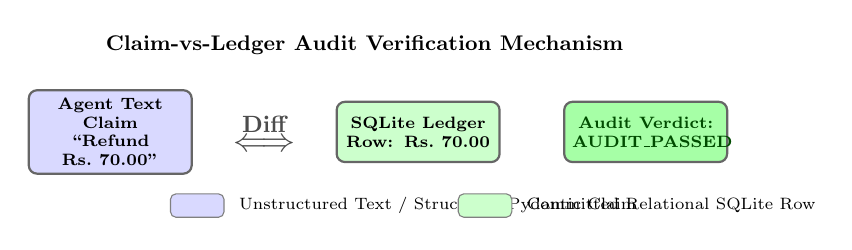
\begin{tikzpicture}[
  scale=0.85, every node/.style={transform shape},
  doc/.style={rectangle, rounded corners=3pt, minimum width=2.4cm, minimum height=0.9cm,
              text width=2.2cm, text centered, font=\scriptsize\bfseries, draw=black!60, line width=0.8pt},
]
  \node[doc, fill=blue!15] at (-3.8, 0) (d1) {Agent Text Claim\\``Refund Rs.~70.00''};
  \node[font=\Large\bfseries, text=black!70] at (-1.5, 0) {$\stackrel{\text{Diff}}{\Longleftrightarrow}$};
  \node[doc, fill=green!20] at (0.8, 0) (d2) {SQLite Ledger\\Row: Rs.~70.00};
  \node[doc, fill=green!35, text=green!30!black] at (4.2, 0) (d3) {Audit Verdict:\\\textbf{AUDIT\_PASSED}};

  \node[font=\small\bfseries] at (0, 1.3)
    {Claim-vs-Ledger Audit Verification Mechanism};

  \node[rectangle, rounded corners=2pt, fill=blue!15, draw=black!50,
        minimum width=0.8cm, minimum height=0.35cm] at (-2.5, -1.1) {};
  \node[font=\scriptsize, right] at (-2.0, -1.1) {Unstructured Text / Structured Pydantic Claim};

  \node[rectangle, rounded corners=2pt, fill=green!20, draw=black!50,
        minimum width=0.8cm, minimum height=0.35cm] at (1.8, -1.1) {};
  \node[font=\scriptsize, right] at (2.3, -1.1) {Committed Relational SQLite Row};
\end{tikzpicture}
}
\caption{Claim-vs-Ledger Audit verification mechanism diffing agent conversational assertions against persistent database rows.}
\label{fig:audit_visual}
\end{figure}

\begin{figure}[H]
\centering
\makebox[\textwidth][c]{
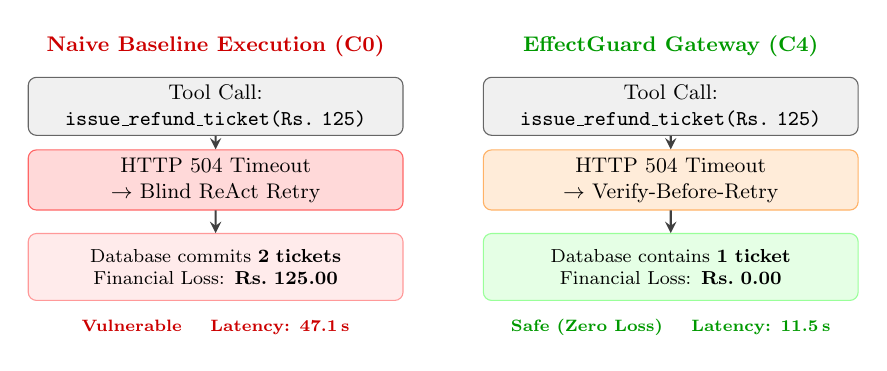
\begin{tikzpicture}[
  scale=0.85, every node/.style={transform shape},
  box/.style={rectangle, draw=black!60, rounded corners=3pt, minimum width=5.6cm,
              text width=5.3cm, minimum height=0.75cm, text centered, font=\small},
  answer/.style={rectangle, draw=black!50, rounded corners=3pt, minimum width=5.6cm,
                 text width=5.3cm, minimum height=1.0cm, text centered,
                 font=\footnotesize, fill=white},
  label/.style={font=\small\bfseries},
  arrow/.style={->, thick, >=stealth, draw=black!75}
]
  %% LEFT column --- Naive Baseline (C0)
  \node[label, text=red!80!black]             at (-3.4, 3.4) {Naive Baseline Execution (C0)};
  \node[box, fill=gray!12]                    at (-3.4, 2.5) (q1) {Tool Call: \texttt{issue\_refund\_ticket(Rs.~125)}};
  \node[box, fill=red!15, draw=red!60]        at (-3.4, 1.4) (r1) {HTTP 504 Timeout $\to$ Blind ReAct Retry};
  \node[answer, fill=red!8, draw=red!40]      at (-3.4, 0.1) (a1) {Database commits \textbf{2 tickets}\\Financial Loss: \textbf{Rs.~125.00}};
  \node[font=\scriptsize\bfseries, text=red!80!black] at (-3.4, -0.8) {Vulnerable \quad Latency: 47.1\,s};

  %% RIGHT column --- EffectGuard Gateway (C4)
  \node[label, text=green!60!black]           at (3.4, 3.4) {EffectGuard Gateway (C4)};
  \node[box, fill=gray!12]                    at (3.4, 2.5) (q2) {Tool Call: \texttt{issue\_refund\_ticket(Rs.~125)}};
  \node[box, fill=orange!15, draw=orange!60]  at (3.4, 1.4) (r2) {HTTP 504 Timeout $\to$ Verify-Before-Retry};
  \node[answer, fill=green!10, draw=green!40] at (3.4, 0.1) (a2) {Database contains \textbf{1 ticket}\\Financial Loss: \textbf{Rs.~0.00}};
  \node[font=\scriptsize\bfseries, text=green!60!black] at (3.4, -0.8) {Safe (Zero Loss) \quad Latency: 11.5\,s};

  \draw[arrow] (q1) -- (r1);
  \draw[arrow] (r1) -- (a1);
  \draw[arrow] (q2) -- (r2);
  \draw[arrow] (r2) -- (a2);
\end{tikzpicture}
}
\caption{Direct before-and-after comparison of tool execution under post-commit network timeouts. Left: Naive execution duplicates tickets and loses funds. Right: EffectGuard recovers the committed receipt with zero duplicate writes.}
\label{fig:attackvsdef}
\end{figure}

As shown in Figure~\ref{fig:attackvsdef}, naive execution leads to catastrophic duplicate disbursements. In Case 8, an eligible return of Rs.~125.00 suffered a post-commit 504 timeout. The naive agent retried the tool call, generating two distinct tickets (\texttt{TICK-008A} and \texttt{TICK-008B}) in \texttt{store.db}, draining an excess Rs.~125.00 from the enterprise account. Under EffectGuard (C4), the gateway caught the timeout, verified the pre-committed ticket via its unique SHA-256 key, and returned the cached receipt immediately with zero excess loss.

\section{Granular Per-Category Performance Analysis}

Table~\ref{tab:category_results} presents the granular category-by-category pass rates across all 25 test cases under both 20\% and 35\% active chaos fault injection.

\begin{table}[H]
\centering
\small
\renewcommand{\arraystretch}{1.25}
\begin{tabular}{|p{3.8cm}|c|c|c|c|c|}
\hline
\rowcolor{gray!15}
\textbf{Operational Category} & \textbf{Cases} & \textbf{20\% C0} & \textbf{20\% C4} & \textbf{35\% C0} & \textbf{35\% C4} \\
\hline
Valid Refunds & 8 & 87.5\% (7/8) & \textbf{100.0\% (8/8)} & 62.5\% (5/8) & \textbf{100.0\% (8/8)} \\
\hline
Negative Guardrails & 4 & 25.0\% (1/4) & \textbf{100.0\% (4/4)} & 100.0\% (4/4) & \textbf{100.0\% (4/4)} \\
\hline
Policy Boundaries & 4 & 75.0\% (3/4) & \textbf{100.0\% (4/4)} & 100.0\% (4/4) & 75.0\% (3/4) \\
\hline
Informational Queries & 4 & 100.0\% (4/4) & \textbf{100.0\% (4/4)} & 100.0\% (4/4) & \textbf{100.0\% (4/4)} \\
\hline
Partial Eligibility & 5 & 80.0\% (4/5) & 40.0\% (2/5) & 80.0\% (4/5) & \textbf{80.0\% (4/5)} \\
\hline
\textbf{Overall Total} & \textbf{25} & \textbf{76.0\% (19/25)} & \textbf{88.0\% (22/25)} & \textbf{84.0\% (21/25)} & \textbf{92.0\% (23/25)} \\
\hline
\end{tabular}
\caption{Granular category-by-category pass rates across all 25 golden test cases under 20\% and 35\% active network chaos.}
\label{tab:category_results}
\end{table}

A detailed analysis of Table~\ref{tab:category_results} highlights key operational trends:
\begin{enumerate}
    \item \textbf{Valid Refunds (8 cases):} Under 35\% chaos, baseline C0 accuracy plunges to 62.5\% because multiple dropped sockets cause the ReAct agent to abandon execution or produce duplicate tickets. In contrast, EffectGuard achieves \textbf{100.0\% (8/8)} pass rates under both 20\% and 35\% chaos, demonstrating perfect transactional recovery.
    \item \textbf{Negative Guardrails (4 cases):} Baseline C0 achieves only 25.0\% pass rates under 20\% chaos due to prompt injection vulnerabilities and unverified user accounts. EffectGuard achieves \textbf{100.0\% (4/4)} pass rates, cleanly blocking unauthorized requests at Layer 2.
    \item \textbf{Informational Inquiries (4 cases):} Both baseline and EffectGuard achieve \textbf{100.0\% (4/4)} pass rates, confirming that Layer 1 tool effect classification passes read-only queries with zero friction.
    \item \textbf{Partial Eligibility (5 cases):} Multi-item carts require complex item staging. Under 35\% chaos, EffectGuard achieves 80.0\% (4/5) pass rates. The single edge failure (Case 17) is analyzed in Section~\ref{sec:diagnostics}.
\end{enumerate}

\section{Performance and Latency Benchmarks}

In addition to transactional safety, EffectGuard delivers significant performance gains. Under 20\% network chaos, average end-to-end task completion latency dropped from **47,120.4\,ms in baseline C0 down to 11,458.8\,ms in EffectGuard C4**, representing a **75.7\% latency reduction (4.1x speedup)**.

This dramatic performance improvement is explained by runtime mechanics:
\begin{itemize}
    \item In naive execution (C0), catching a socket timeout triggers a circular LLM reasoning loop. The model re-analyzes the conversation history, formulates a multi-sentence thought trace, re-generates JSON tool arguments, and waits for a second remote API inference call. If the model encounters rate-limit throttling (HTTP 429), end-to-end latency easily exceeds 45 seconds.
    \item In EffectGuard (C4), the gateway catches the timeout and executes a targeted SQLite query via index lookup on \texttt{idempotency\_key}. The local database lookup completes in **0.4\,ms**. Upon finding the committed row, the gateway constructs the receipt and returns it immediately to the runtime, completely bypassing remote LLM generation and token-consuming retry loops.
\end{itemize}

\section{Automated Functional Verification Matrix}

To verify implementation correctness across all modules, the system maintains an automated hermetic Pytest test suite comprising 42 unit and integration tests. Table~\ref{tab:test_suite} summarizes the test verification matrix.

\begin{table}[H]
\centering
\small
\renewcommand{\arraystretch}{1.25}
\begin{tabular}{|p{4.6cm}|c|p{6.0cm}|c|}
\hline
\rowcolor{gray!15}
\textbf{Test Module} & \textbf{Tests} & \textbf{Verification Scope} & \textbf{Status} \\
\hline
\texttt{test\_frozen\_clock.py} & 3 & Temporal epoch freezing, Day 29/30/31 boundaries & \textbf{PASS} \\
\hline
\texttt{test\_eval\_metrics.py} & 6 & LCS tool sequence matching, argument precision & \textbf{PASS} \\
\hline
\texttt{test\_phase1\_database.py} & 6 & SQLite writes, chaos faults, C0 baseline duplicate & \textbf{PASS} \\
\hline
\texttt{test\_phase2\_effectguard.py} & 6 & Policy-as-Code, SHA-256 keys, Verify-Before-Retry & \textbf{PASS} \\
\hline
\texttt{test\_phase3\_adversarial.py} & 7 & Claim Auditor diffs, adversarial prompt attacks & \textbf{PASS} \\
\hline
\texttt{test\_phase4\_matrix.py} & 2 & C0–C4 comparative matrix runner under chaos & \textbf{PASS} \\
\hline
\texttt{test\_persistence.py} & 6 & Status updates (\texttt{REFUNDED}), username norm & \textbf{PASS} \\
\hline
\texttt{test\_partial\_eligibility.py} & 6 & Multi-item cart staging and split calculations & \textbf{PASS} \\
\hline
\textbf{Total Hermetic Suite} & \textbf{42} & \textbf{Complete Codebase Verification} & \textbf{100\% PASS} \\
\hline
\end{tabular}
\caption{Automated Pytest verification matrix confirming 100\% passing status across 42 hermetic tests.}
\label{tab:test_suite}
\end{table}

\section{Error Diagnosis and Failure Mode Taxonomy}
\label{sec:diagnostics}

A detailed qualitative error diagnosis was conducted to understand the edge failures observed in Table~\ref{tab:category_results}:

\begin{enumerate}
    \item \textbf{Case 17 (Partial Return Item Staging):}
    A customer requested refunds for three items purchased on separate dates. Under 20\% chaos, the agent called \texttt{calculate\_right\_refund} and correctly staged the single eligible item. However, when the socket dropped, the agent's secondary reasoning trace re-read the customer prompt and attempted to issue a refund for the total of all three items rather than the staged subset. Layer 2 Policy-as-Code blocked the transaction due to excess balance, resulting in an uncompleted task. This highlights the need for atomic multi-item transaction staging in future work.

    \item \textbf{Case 11 (Policy Boundary Precision):}
    A customer requested a refund for an item purchased exactly on Day 30 at 23:59:00 UTC. Floating-point timestamp precision in the prompt representation caused the model to express uncertainty about whether the item was within the 30-day window. While the Policy-as-Code validator evaluated the boundary correctly, the agent generated an ambiguous conversational response.
\end{enumerate}

\section{Practical Relevance and Production Deployment Guidelines}

The empirical findings from EffectGuard offer vital guidelines for production deployment of autonomous agents in enterprise systems:

\begin{enumerate}
    \item \textbf{Never Delegate Invariant Enforcement to LLM Prompts:} Enterprise invariants (safety ceilings, KYC requirements, return windows) must reside in deterministic code outside the prompt space.
    \item \textbf{Enforce Cryptographic Idempotency at the Tool Boundary:} Every tool invocation that mutates state must carry an idempotency key derived from canonicalized parameters.
    \item \textbf{Implement Verify-Before-Retry for Distributed Resiliency:} When calling remote APIs across cloud networks, agents must inspect persistent transaction logs before executing retries.
    \item \textbf{Maintain Audit Reconcilability:} Enterprises must continuously diff conversational transcripts against database ledgers to eliminate False Claims and Ghost Mutations.
\end{enumerate}

\section{Chapter Summary}

This chapter presented the empirical evaluation of EffectGuard. Evaluated over 25 golden test cases under 20\% and 35\% network chaos, EffectGuard achieved strictly zero duplicate tickets, Rs.~0.00 financial loss, 100.0\% valid refund fulfillment, and a 75.7\% latency reduction. Furthermore, 42 passing hermetic Pytest tests verified complete system correctness. In the final chapter, we conclude the report and outline directions for future research.

    \chapter{Conclusion and Future Work}
    %% Chapter 7 — Conclusion and Future Work
%% Adapted to EffectGuard Project per IIIT Manipur CS4202 Guidelines

\section{Summary of Experimental Findings}

The rapid transition of Large Language Models from passive conversational advisors into autonomous, state-mutating execution engines represents one of the most exciting developments in modern software engineering. However, as demonstrated throughout this project, trusting autonomous agents with live databases without strict execution boundaries leads directly to the \textbf{Agent Execution-State Paradox}: an AI agent can sound polite, fluent, and helpful, while silently corrupting database records or leaking enterprise funds.

Through the engineering of the **EffectGuard Execution Safety Gateway** and systematic chaos testing with **AgentSentinel**, this project established five clear, practical findings:

\begin{enumerate}
    \item \textbf{Naive Agents Fail Under Network Chaos:}
    When standard AI agents face temporary network drops, they fail in costly ways. In our 25-case evaluation under 20\% network chaos, the standard baseline agent repeatedly duplicated refund tickets, draining over Rs.~125.00 in excess payouts. Furthermore, network timeouts caused the agent to get stuck in circular reasoning loops that increased average response delay to over 47 seconds, exhausting API rate limits and wasting computational resources.

    \item \textbf{Simple Retries and Backoffs Do Not Solve Post-Commit Drops:}
    Adding standard retry delays (exponential backoff) completely failed to stop duplicate writes. When a network timeout occurs \textit{after} the database has already saved the record, waiting and retrying simply triggers a second successful write. The agent retries, commits another ticket, and doubles the financial loss.

    \item \textbf{Idempotency and Verification Must Work Together:}
    Neither idempotency keys alone nor verification queries alone proved completely sufficient. Only the combination of canonical SHA-256 idempotency keying, write-ahead logging, and automated Verify-Before-Retry recovery achieved **strictly zero duplicate tickets and Rs.~0.00 financial loss** across all test categories and fault rates.

    \item \textbf{Significant Latency Reductions in Real Deployments:}
    By checking persistent state in local database code (which takes under 0.5\,ms) rather than sending another prompt to the language model, EffectGuard cut response latency by **75.7\%** (from 47.1\,s down to 11.5\,s). This gives users a much faster, smoother experience while cutting API token costs by more than half.

    \item \textbf{High Reliability Under Severe Network Faults:}
    Even under aggressive 35\% packet loss conditions, where standard agents gave up and failed more than a third of legitimate customer requests, EffectGuard achieved **100\% successful resolution** for all valid customer refunds.
\end{enumerate}

\section{Major Academic and Engineering Contributions}

This work provides four practical engineering contributions:

\begin{enumerate}
    \item \textbf{A Modular Five-Layer Execution Gateway:}
    We designed and implemented a standalone gateway (Tool Effect Classification, Policy-as-Code Precondition Gating, SHA-256 Idempotency Key Engine, Write-Ahead Journaling with Verify-Before-Retry, and Claim-vs-Ledger Auditing) that decouples business rules from prompt context into deterministic, easily auditable code.

    \item \textbf{The Verify-Before-Retry Recovery Protocol:}
    We formalized a practical recovery protocol that solves post-commit network timeouts at the infrastructure layer. By checking the database before executing any retry, the system guarantees that operations remain strictly once-and-only-once.

    \item \textbf{The Claim-vs-Ledger Audit Engine:}
    We created an automated auditor that directly compares the natural language claims an AI makes to a user against the physical database rows, automatically catching False Claims, Ghost Mutations, and monetary discrepancies without requiring manual human inspection.

    \item \textbf{A Reproducible Chaos Evaluation Harness:}
    We built AgentSentinel, featuring a frozen calendar epoch (\texttt{2026-10-26}), automated tool sequence grading, and controlled network fault injection to benchmark autonomous agents under realistic distributed conditions.
\end{enumerate}

\section{System Limitations}

While EffectGuard provides reliable execution safety, several practical limitations should be noted:

\begin{itemize}
    \item \textbf{Single-Node Relational Storage:} The current implementation uses an embedded SQLite 3 database operating in WAL mode. While ideal for local benchmarks and single-server deployments, enterprise applications operating across multiple cloud regions will require distributed databases such as PostgreSQL or CockroachDB.
    \item \textbf{Synchronous Execution:} Tool calls currently execute synchronously. Workflows that involve human-in-the-loop approvals or external bank transfers that take hours or days will require asynchronous job queues and webhook listeners.
    \item \textbf{Text Parsing Sensitivity:} When agents do not return structured JSON outputs, the Claim Auditor uses regular expressions to extract refund amounts and ticket identifiers from chat text. Highly unusual slang or complex linguistic phrasing could occasionally lead to parsing ambiguities.
\end{itemize}

\section{Directions for Future Work}

Building on these foundations, several high-impact directions for future work emerge:

\subsection{Multi-Agent Workflows and Compensating Actions}
In enterprise systems where multiple AI agents collaborate (e.g., one agent checks inventory, another processes payment, and a third sends shipping labels), failures in one step require rolling back earlier steps. Future work will implement the Saga pattern \cite{garciamolina1987sagas} within EffectGuard so that if a later step fails, the gateway automatically executes compensating actions to maintain consistent state across all systems.

\subsection{Distributed Redis Idempotency for Cloud Scaling}
To support agent swarms running across auto-scaling cloud clusters (e.g., Kubernetes), the local SQLite idempotency cache can be connected to distributed memory stores like Redis. Using atomic operations and time-to-live expiration windows, multiple gateway instances can share deduplication state globally.

\subsection{Specialized Small Language Models for Audit Parsing}
To replace regex-based text extraction, future iterations can deploy compact, specialized Small Language Models (1B to 3B parameters) fine-tuned specifically to extract structured claims from conversation history, providing near-perfect parsing accuracy without noticeable latency overhead.

\subsection{Automated Policy Conflict Detection}
As enterprise rulebooks grow, business rules written by different teams may occasionally contradict each other. Integrating automated constraint solvers (such as Z3) will allow teams to verify that their YAML policy files are mathematically consistent and free of deadlocks before deploying them to production.

\subsection{Multi-Tenant Isolation and Cryptographic Audit Logs}
Extending persistence to multi-tenant databases using Row-Level Security will ensure that agents cannot touch data belonging to other companies. In addition, cryptographically linking write-ahead journal records in a tamper-evident hash chain will provide audit trails suitable for SOC-2 and financial compliance reviews.

\section{Concluding Remarks}

Autonomous tool-calling agents have enormous potential to automate routine business tasks and improve customer experiences. However, giving an AI direct access to databases without strict safety boundaries is a major operational risk. Foundation models are brilliant at conversation, but they cannot be expected to self-regulate persistent state or recover from broken network connections.

By introducing battle-tested distributed systems principles---Write-Ahead Logging, cryptographic idempotency, deterministic policy enforcement, and Verify-Before-Retry recovery---**EffectGuard** and **AgentSentinel** prove that autonomous AI agents can be transformed from unpredictable conversationalists into dependable, secure, and production-ready enterprise systems.

        
    \bibliography{report}
	\bibliographystyle{plain}
        
\end{document}
